
\usection{Análisis inicial del sistema de monitoreo acústico para generar alertas en casos de emergencia.}

Desde el planteamiento del proyecto se identificó como un problema social relevante la detección de situaciones de emergencia en el hogar, especialmente para personas más expuestas a quedar desatendidas ante situaciones de vulnerabilidad, como adultos mayores que viven solos o personas con condiciones médicas que limitan su movilidad. Estudios como el de \cite{bezold2021sensor}, destacan la prevalencia de caídas y emergencias médicas en estos grupos. Esta realidad evidencio la necesidad de un sistema de monitoreo que funcione de manera autónoma y discreta, sin depender de la intervención del usuario debido a su posible incapacidad para interactuar con un dispositivo durante una emergencia.

Para el análisis  inicial del sistema, se comenzó con la revisión de literatura científica y técnica relacionada con la identificación y caracterización de eventos acústicos. Se prestó especial atención a estudios que abordaran la implementación de sistemas en dispositivos de Edge Computing.

Esta revisión incluyó estudios sobre el procesamiento de señales de audio y modelos de aprendizaje automático aplicados al reconocimiento de sonidos. Se encontró que era posible representar una señal de audio gráficamente como un espectrograma, que es una representación visual del sonido en función del tiempo y la frecuencia, donde la intensidad se codifica con color o brillo. Esto significa que la información necesaria para distinguir eventos sonoros, que se encuentra en las complejas estructuras de frecuencias del audio, podía ser interpretada mediante técnicas de análisis de imágenes.

Esto sugirió que, para una caracterización significativa del sonido, la estrategia de solución debía enfocarse en la Clasificación de Eventos Acústicos. En este contexto, la Inteligencia Artificial, particularmente las Redes Neuronales Convolucionales (CNN), se presentó como el enfoque más adecuado para procesar y etiquetar la información compleja contenida en la estructura de frecuencias (el espectrograma). Este enfoque se ve respaldado por la literatura; por ejemplo, investigaciones en el diagnóstico de fallos de maquinaria han demostrado la efectividad de utilizar representaciones espectrales, como el Mel Spectrogram y el Scalogram, para la detección automática de anomalías acústicas mediante arquitecturas de Deep Learning \cite{tran2020drill}.

Sabiendo que la clasificación de eventos acústicos conforma un componente necesario para la solución se identificó una limitante, la clasificación por sí sola no resolvía el problema, debido a la alta variabilidad del entorno sonoro domestico. No es lo mismo caracterizar sonidos en un entorno donde el comportamiento de las senales de audio es estable y predecible (como en una maquina), que en un hogar donde los sonidos son altamente dinámicos y contextuales. Es decir, la clasificación de eventos aislados no proporciona suficiente contexto para determinar si un evento es crítico o no. Por ejemplo, escuchar un grito sin contexto no permite determinar si es una situación de emergencia o una expresión normal de alegría o sorpresa. En otras palabras, la clasificación de eventos aislados es insuficiente para detectar situaciones críticas, ya que carece del contexto necesario para interpretar adecuadamente los eventos sonoros.

Ante esta limitante y asumiendo que las emergencias son eventos poco frecuentes y atípicos dentro del patrón de actividad sonora normal del hogar, se consideró la necesidad de analizar el comportamiento temporal de los eventos acústicos. Esto implicaba no solo clasificar los sonidos, sino también entender cómo estos eventos se distribuían a lo largo del tiempo para identificar patrones normales y detectar desviaciones significativas que pudieran indicar una emergencia.

Para abordar la necesidad del análisis de secuencias temporales, se revisaron estudios previos sobre predicción de eventos basados en series temporales. El uso de modelos predictivos como ARIMA, SARIMA o Prophet es una práctica establecida en la literatura para el desarrollo de sistemas de alerta temprana mediante el análisis y la predicción de patrones temporales \citeauthor{mora2023analisis} \citeyear{mora2023analisis}. Estos modelos se perfilaban como una estrategia para establecer umbrales de predicción sobre la secuencia de eventos acústicos. El objetivo era determinar qué tan ``típica'' resultaba la ocurrencia en un momento dado, sirviendo así como un detector de patrones de comportamiento anómalo.

En función del analisis realizado, se procedio a definir los requerimientos del sistema de monitoreo acústico para la detección de emergencias en el hogar. La verificacion de los mismos se encuentra en la tabla \ref{tab:requerimientos_sistema_acustico}

\usubsection{Requerimientos Funcionales}

\begin{enumerate}
      \item El sistema debe capturar el audio ambiental de forma continua a través de los micrófonos.
      \item El sistema debe procesar el audio capturado para su caracterización.
      \item El sistema debe caracterizar el perfil de la actividad acústica ``típica'' del entorno, basado en la estacionalidad de los eventos sonoros clasificados.
      \item El sistema debe procesar y comparar la actividad sensada de manera inmediata con el perfil de normalidad para detectar patrones anómalos con la mínima latencia posible.
      \item El sistema debe enviar notificaciones de emergencia a una lista de contactos predefinidos si se detecta una anomalía o grito de auxilio.
\end{enumerate}

\usubsection{Requerimientos no funcionales}

\begin{enumerate}
      \item El sistema debe procesar y analizar los datos de audio en el borde (edge) sin almacenar las grabaciones de audio bruto ni información personal identificable.
      \item El sistema debe ser capaz de integrar de manera flexible nuevos dispositivos de procesamiento (hardware) y/o de captura (micrófonos).
      \item El sistema debe contar con una característica de inicio automático después de cualquier corte de energía o reinicio forzado.
      \item El sistema debe tener un diseño modular que simplifique y agilice las tareas de mantenimiento y actualización de sus componentes.
\end{enumerate}

\usection{Procedimiento Metodológico}

\usubsection{Primera Iteracion}

      \begin{figure}[ht!]
            \centering
            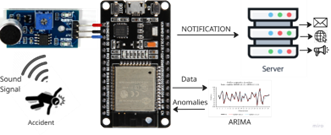
\includegraphics[width=0.65\textwidth]{Arquitectura/I1.png}
            \caption{Prototipo basado en ESP32 y detección de intensidad de sonido}
            \label{fig:prototipo1}
      \end{figure}

El objetivo principal de la primera iteración fue validar la hipótesis de que se podían detectar anomalías en el comportamiento sonoro del entorno mediante el análisis de series temporales de intensidad. La estrategia consistió en utilizar un modelo estadístico para predecir el comportamiento sonoro "normal", de modo que cualquier diferencia significativa entre el valor predicho y el valor real observado fuera clasificada como una anomalía. El principal riesgo identificado en esta etapa fue la capacidad del modelo estadístico para funcionar adecuadamente en un entorno tan dinámico y variable como el doméstico.

Los componentes con los que contó esta iteración fueron un microcontrolador ESP32 y un micrófono que capturaba la intensidad de sonido. Véase en la figura \ref{fig:prototipo1}. Esta serie temporal de niveles de intensidad sonora fue procesada por un modelo ARIMA (AutoRegressive Integrated Moving Average) para predecir el comportamiento esperado. Si la diferencia entre el valor predicho y el valor real superaba un umbral predefinido, se generaba una alerta.

El diseño del prototipo para probar este enfoque se inspiró en metodologías documentadas para sistemas IoT \cite{luis2024desarrollo} y consistió en un dispositivo de captura basado en un microcontrolador ESP32, que transmitía los datos a un servidor local (Raspberry Pi 4) para su análisis con el modelo ARIMA.Sin embargo, durante la fase de evaluación, este enfoque demostró ser fundamentalmente inviable. El problema de fondo no fue solo que el modelo ARIMA tuviera limitaciones funcionales, sino que su propio proceso de parametrización resultó ser incompatible con la naturaleza del problema de investigación.

La parametrización de ARIMA (basada en los parámetros $p, d, q$) busca definir una estructura de dependencia y estacionalidad fija en los datos. En un entorno doméstico, la estacionalidad de los eventos acústicos es altamente variable y depende de múltiples factores contextuales, como la hora del día, el día de la semana, o eventos imprevistos. Esta variabilidad hace que sea extremadamente difícil definir parámetros fijos que puedan capturar adecuadamente los patrones normales de comportamiento sonoro para cualquier entorno, confirmando el riesgo inicial sobre la inestabilidad.

La principal limitación funcional de esta iteración fue la incapacidad de distinguir entre diferentes tipos de anomalías, ya que el modelo solo identificaba desviaciones en la intensidad del sonido sin considerar su naturaleza o contexto (e.g., una anomalía de volumen alto podía ser tanto una alarma como un evento crítico).

Con estas limitaciones identificadas, se decidió avanzar hacia una segunda iteración que abordara estos desafíos.

\usubsection{Segunda Iteracion}

      \begin{figure}[ht!]
            \centering
            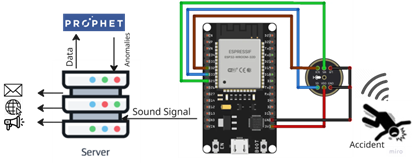
\includegraphics[width=0.85\textwidth]{Arquitectura/I2.png}
            \caption{Diseño de prototipo de esp32 con micrófono de señales de audio y prophet}
            \label{fig:prototipo2}
      \end{figure}

      En la Segunda Iteración, el objetivo fue superar la rigidez del modelo ARIMA, que resultó incompatible con la dinámica del entorno doméstico, manteniendo el enfoque de análisis de series temporales. La principal limitación, que se convirtió en el riesgo metodológico de esta etapa, radicaba en la pregunta de si la naturaleza dinámica y no estacionaria de los eventos domésticos podría ser modelada adecuadamente por cualquier librería de pronóstico que requiriera patrones estables. Se mantuvo la arquitectura de hardware de Edge Computing basada en el microcontrolador ESP32 y se aplicaron mejoras en la captura de datos. Se integraron micrófonos omnidireccionales INMP441 para asegurar una captura de señales acústicas de alta fidelidad, véase en la figura \ref{fig:prototipo2}. A nivel de software, se reemplazó el modelo ARIMA por Prophet, una librería de pronóstico de series temporales desarrollada por Facebook, elegida por su capacidad para manejar estacionalidad y tendencias complejas, buscando mayor flexibilidad para modelar el entorno.
      
      El modelo Prophet logró ajustarse eficazmente a las variaciones periódicas del sonido ambiental, como los patrones de ruido diurnos y nocturnos. Sin embargo, durante las pruebas se identificó una limitación crítica, confirmando el riesgo inicial asociado al pronóstico: el mecanismo interno del modelo para suavizar datos e identificar tendencias a largo plazo provocaba que se descartaran los eventos de corta duración y alta amplitud de interés. Sonidos instantáneos como un golpe, un grito o la rotura de un cristal eran filtrados y no generaban alertas, ya que no formaban parte de un patrón estacional o de una tendencia predecible. Esta observación llevó a la conclusión definitiva de que el enfoque de pronóstico de series temporales, independientemente del modelo (ARIMA o Prophet), no era el adecuado para el objetivo del proyecto. El problema no era predecir la evolución del nivel de ruido, sino la detección de eventos atípicos e instantáneos basados en el contenido acústico. Por lo tanto, el problema se redefinió como uno de detección de anomalías en tiempo real basada en la caracterización de la señal. Para implementar esta nueva estrategia, se propuso un enfoque basado en una arquitectura de redes neuronales (Deep Learning). 

      La Planificación de la siguiente iteración se centró en la implementación de un modelo de clasificación acústica para caracterizar los eventos sonoros, seguido de un análisis temporal de las secuencias de eventos para detectar anomalías basadas en patrones de comportamiento. 
      

\usubsection{Tercera iteración}


El objetivo de esta tercera iteración fue abordar la necesidad de la caracterización semántica del sonido que se identificó como limitación crítica en las etapas previas. Inicialmente, la estrategia se centró en el desarrollo de un modelo de clasificación personalizado a partir de un conjunto de datos propio. El plan consistía en capturar y etiquetar una colección de sonidos de emergencia para entrenar una red neuronal diseñada específicamente para los escenarios de interés del proyecto.El principal riesgo metodológico de esta etapa fue la viabilidad de la adquisición de datos. Se asumió el riesgo de que la construcción de un dataset lo suficientemente vasto y diverso para garantizar la robustez y generalización del clasificador resultara inviable para los recursos del proyecto. A pesar de este riesgo, el diseño de hardware de Edge Computing se mantuvo para el desarrollo, enfocado en el procesamiento local de las señales.

Sin embargo, a medida que avanzaba el desarrollo, la investigación sobre la robustez de los clasificadores acústicos reveló la verdadera magnitud del desafío. Se hizo evidente que para que un modelo pudiera generalizar y operar de manera fiable, necesitaría ser entrenado con un volumen de datos masivo. La literatura académica confirma que la efectividad de los modelos de aprendizaje profundo para audio depende directamente de la escala y diversidad de los datos, requiriendo a menudo millones de ejemplos para capturar la enorme variabilidad de los sonidos del mundo real \cite{gemmeke2017audio}. La tarea de construir un dataset de esa magnitud, confirmando el riesgo inicial, era logísticamente inviable para el proyecto.

Fue precisamente durante esta etapa de investigación que se identificó YAMNet, una arquitectura de clasificación acústica ya pre-entrenada por Google. Este modelo fue entrenado sobre el corpus AudioSet, un extenso conjunto de datos que, como describen \citeauthor{gemmeke2017audio} \citeyear{gemmeke2017audio}, contiene más de dos millones de clips de audio de $10$ segundos etiquetados a partir de una ontología de $527$ clases de eventos sonoros. El descubrimiento de YAMNet ofreció una solución directa al problema de la adquisición de datos a gran escala que se había identificado como el principal obstáculo.Ante esta situación, continuar con el desarrollo de un modelo propio habría significado un esfuerzo redundante. Por lo tanto, se tomó la decisión de descartar el enfoque personalizado y pivotar hacia la integración de YAMNet. 

Esta medida representa una aplicación práctica del paradigma de aprendizaje por transferencia (transfer learning), que permite aprovechar el conocimiento de un modelo ya entrenado en un gran dataset para resolver un problema específico, tal como analizan \citeauthor{pons2019deep} \citeyear{pons2019deep} en su trabajo sobre el impacto del tamaño del dataset en audio. Este pivote tecnológico permitió enfocar los recursos restantes del proyecto en la implementación del sistema final sobre una base tecnológica robusta y ya validada, y superar la limitación de la falta de contexto que afectó a las iteraciones basadas en series temporales.

\usubsection{Cuarta Iteración}

      \begin{figure}[ht!]
            \centering
            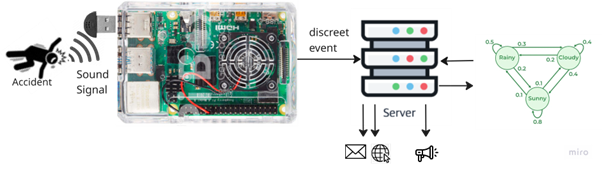
\includegraphics[width=0.85\textwidth]{Arquitectura/I4.png}
            \caption{Prototipo con Raspberry Pi, Yamnet y Cadenas de Markov}
            \label{fig:prototipo4}
      \end{figure}

      En esta cuarta iteración del prototipo, se migró la lógica de procesamiento desde el ESP32 hacia una Raspberry Pi, con mayor capacidad computacional. Se integraron micrófonos digitales de rango completo, capaces de capturar la senal de audio completa, lo que permitió acceder a un contenido espectral  completo. Véase en la figura \ref{fig:prototipo4}.

      Con esta infraestructura, se incorporó YAMNet, un modelo de clasificación de audio en tiempo real basado en redes neuronales convolucionales entrenado con el dataset AudioSet de Google. YAMNet permite detectar y clasificar una gran variedad de eventos acústicos o (más de 500 categorías) como gritos, portazos, pasos, objetos cayendo, entre otros. Esta capacidad permitió dar un salto importante en la interpretación contextual del entorno sonoro.

      No obstante, Si bien YAMNet ofrecía una detección puntual efectiva de eventos sonoros, surgió la necesidad de dotar a dichos eventos de un significado secuencial y contextual. Para atender esta limitación, se optó por integrar un módulo de modelado probabilístico basado en cadenas de Márkov, con el fin de analizar la secuencia temporal de eventos y determinar si un patrón resultaba coherente con el comportamiento normal del entorno o, por el contrario, representaba una posible anomalía.

      La decisión de emplear cadenas de Márkov estuvo fundamentada en dos aspectos principales: por un lado, en la existencia de estudios previos donde este tipo de modelos han sido utilizados para la detección de anomalías en secuencias temporales, destacando por su capacidad de representar probabilísticamente las transiciones entre estados inmediatos. En particular, investigaciones como la de \citeauthor{boldt2020anomaly} \citeyear{boldt2020anomaly}, muestran cómo las cadenas de Márkov permiten identificar patrones irregulares en secuencias de eventos al modelar las transiciones esperadas y comparar estas con la realidad observada. Por otro lado, la elección también estuvo motivada por la recomendación del profesor de estadistica Omar Castro, quien sugirió explorar este enfoque como un primer acercamiento al modelado secuencial de los eventos detectados.

      No obstante, también surgieron limitaciones importantes. Si bien éramos capaces de detectar situaciones potencialmente peligrosas a partir de categorías específicas identificadas por YAMNet, el intento de modelar secuencias completas de eventos mediante cadenas de Márkov resultó ineficaz, ya que se quedaba saltando en ciclos infinitos de cambios de estado, por ejemplo (luego de Habla el siguiente evento mas probable era Habla). Estas cadenas se limitan a representar transiciones entre estados inmediatos, es decir, predicen solo el evento más probable siguiente, sin tener en cuenta el historial completo de eventos previos.

      Intentar forzar el modelado de secuencias más largas con este enfoque llevó a comportamientos problemáticos, como ciclos repetitivos sin resolución lógica, o secuencias que carecían de coherencia contextual, especialmente cuando el espacio de eventos posibles crecía. Esta rigidez estructural impidió representar adecuadamente escenarios más complejos o ambiguos, donde la interpretación depende no solo del último evento detectado, sino de una serie de interacciones acústicas encadenadas en el tiempo.

      Este hallazgo marcó un punto de inflexión en el desarrollo del sistema, motivando la exploración de enfoques más robustos y dinámicos, capaces de capturar dependencias de largo plazo en secuencias acústicas. En particular, se consideraron modelos como LSTM (Long Short-Term Memory) y transformers , que permiten aprender patrones secuenciales con memoria y contexto más amplio.


\usubsection{Quinta Iteración}

      En esta quinta iteración, nos enfocamos en el desarrollo de una solución más robusta para la detección de anomalías, como respuesta a las limitaciones encontradas con las cadenas de Markov. Para ello, basamos nuestro enfoque en el trabajo de \citeauthor{reis2025edge} \citeyear{reis2025edge}, cuya investigación se centra en arquitecturas de Inteligencia Artificial en el borde (Edge AI) para el monitoreo en tiempo real. Específicamente, su estudio valida el uso de dos tecnologías que adoptamos: Isolation Forest (IF), un modelo para la detección de eventos anomalos basado en arboles, y un Long Short-Term Memory Autoencoder (LSTM), una red neuronal para el análisis de patrones secuenciales complejos.

      Para la implementación de estos modelos en nuestro sistema, se replicaron las configuraciones de hiperparámetros validadas en dicho estudio para asegurar el rendimiento en la Raspberry Pi.

      En el caso del Isolation Forest, adoptamos los hiperparámetros del estudio, configurando el modelo con 100 árboles ($n_estimators$) y un parámetro de contaminación del 3\%. Este último valor asume una proporción esperada de anomalías en nuestros datos, alineándose con los escenarios simulados en la investigación de referencia.

      El segundo modelo implementado es un LSTM Autoencoder, una arquitectura de red neuronal no supervisada especialmente eficaz para la detección de anomalías en datos secuenciales \cite{malhotra2015long}. Su objetivo es aprender una representación comprimida de los patrones ``normales'' presentes en los datos de entrenamiento para luego identificar desviaciones significativas. De igual manera, se adoptaron los hiperparámetros recomendados por \citeauthor{reis2025edge} \citeyear{reis2025edge}, que incluyen un tamaño de lote de 32 y 50 épocas de entrenamiento. La arquitectura específica del modelo consta de 3 capas LSTM en el codificador y 3 capas LSTM en el decodificador, con tamaños de capa decrecientes de 32, 16 y 8 unidades respectivamente. y activacion del ReLu para ajustar la tasa de aprendizaje y evitar el sobreajuste.
      Para el desarrollo y aplicación del modelo, se adoptó un enfoque metodológico inspirado en el trabajo de \citeauthor{reis2025edge} \citeyear{reis2025edge}, el cual se estructuró en un proceso de tres etapas: preparación de los datos, construcción y entrenamiento de la arquitectura, y definición del mecanismo de detección.

      \begin{enumerate}
            \item Preparación de los Datos:
                  Para que nuestro modelo LSTM pudiera interpretar los datos de los eventos, fue necesario ``traducirlos'' a un formato numérico que la red neuronal pudiera procesar. Este paso es crucial, ya que el modelo no entiende de fechas o etiquetas de texto por sí mismo; solo trabaja con números y mientras mas sentido y consistencia tengan esos números, mejor podrá aprender.
                  Por ejemplo, si convertimos los días de la semana a números (domingo=0, lunes=1, ..., sábado=6), el modelo interpretaría que el sábado (6) y el domingo (0) son valores muy distantes, cuando en realidad son adyacentes. Este tipo de malentendido impide que la red aprenda patrones que ocurren en la transición del fin de semana.
                  Para resolver este problema, el enfoque consiste en representar las variables temporales de una manera que refleje su naturaleza cíclica. En lugar de ver el tiempo como una línea recta, lo tratamos como un círculo, similar a las manecillas de un reloj. Esto se logra mediante funciones matemáticas (seno y coseno) que asignan a cada instante una coordenada única en un círculo. De esta forma:
                  El sábado queda matemáticamente ``cerca'' del domingo.
                  Las 23:59 quedan justo al lado de las 00:00. Vease el Apendice A
                  Este preprocesamiento es fundamental, pues permite que el modelo LSTM capture patrones de comportamiento continuos y lógicos, como los que ocurren durante la madrugada o en el cambio de un día para otro.
                  Convirtiendo Categorías en Señales Claras
                  De manera similar, el modelo no puede procesar etiquetas de texto como ``uso de microondas'' o ``sensor de movimiento''. Un error común sería asignarles un número a cada una (ej: microondas=1, sensor=2), ya que esto crearía una falsa relación matemática (como si el ``sensor'' fuera el doble del ``microondas'').
                  La solución es una técnica llamada One-Hot Encoding. Funciona como un panel de interruptores, donde cada evento posible tiene su propio interruptor.
                  Cuando ocurre un evento, su interruptor se ``enciende'' (toma el valor de 1) mientras que todos los demás permanecen ``apagados'' (con valor de 0). De esta forma, el modelo recibe una señal clara y sin ambigüedades sobre qué evento específico sucedió, sin crear jerarquías o relaciones numéricas que no existen.
                  Finalmente, el verdadero potencial de un modelo LSTM es su capacidad para entender el contexto. Un evento aislado, como ``se enciende una luz'', no dice mucho. Pero si ocurre dentro de una ``historia'' o secuencia como ``sensor de movimiento activado → se abre la puerta → se enciende la luz'', el patrón es mucho más revelador.
                  Por esta razón, en lugar de analizar los eventos de forma individual, los agrupamos en secuencias superpuestas de una longitud fija (por ejemplo, 10 eventos consecutivos). Es como pasar de ver fotografías individuales a ver pequeños videoclips.
                  Al entregarle los datos en este formato, el modelo LSTM no solo aprende ``qué'' pasó, sino ``en qué orden'' y ``en relación con qué'' otros eventos ocurrieron, permitiéndole así aprender los patrones complejos que definen un comportamiento normal. Con los datos ya ``traducidos'' a este formato numérico, cíclico y secuencial, el modelo está listo para comenzar su fase de entrenamiento.

            \item Arquitectura del Modelo: Utilizamos un tipo especial de red neuronal llamado Autoencoder LSTM.
                  La idea es bastante intuitiva. En lugar de predecir un valor futuro, el objetivo de un autoencoder es aprender a reproducir su propia entrada.
                  Podemos imaginarlo como intentar crear una figura circular con un lápiz y un compas, normalmente lo hariamos con el compas y el resultado es bastante predecible, pero al hacerlo a mano, el resultado va variar.
                  Nuestro modelo funciona igual, se le entrena para ser un experto en  reconstruir secuencias de eventos normales. Cuando se encuentra con una secuencia anómala, su reconstrucción es de mala calidad, y ese ``error de reconstrucción'' es la señal que nos alerta de una anomalía.
                  La arquitectura del autoencoder se divide en dos partes simétricas:
                  El Codificador (El Resumidor): Esta primera mitad de la red toma la secuencia de entrada (nuestro ``videoclip'' de 10 eventos) y la comprime progresivamente en una representación mucho más pequeña y densa. Es como si leyera un párrafo completo y lo resumiera en una sola idea clave. En nuestro caso, dos capas LSTM reducen la dimensionalidad de 32 a 16 bits, creando esa ``idea'' o resumen.
                  El Decodificador (El Reconstructor): Esta segunda mitad toma la idea clave generada por el codificador y realiza el proceso inverso: intenta reconstruir la secuencia original de 10 eventos con la mayor fidelidad posible. Actúa como un espejo del codificador, expandiendo la representación de 16 de vuelta a 32 bits.
                  Para mejorar la robustez del modelo y evitar que simplemente ``memorice'' los datos de entrenamiento, se incluyeron capas de Dropout. Estas capas ``apagaban'' aleatoriamente algunas neuronas durante el entrenamiento, forzando al modelo a aprender patrones más generales y significativos del comportamiento normal.

            \item Entrenamiento y Detección:
                  Una vez definida la arquitectura, el modelo entra en la fase de entrenamiento, que es donde aprende el comportamiento ``normal''. El objetivo del entrenamiento es simple, hacer que el modelo sea bueno reconstruyendo las secuencias de eventos normales y muy malo haciendo lo mismo con las anómalas. Para ello, se le alimenta con una serie constante de datos que representan la normalidad.
                  El modelo procesa los datos en un ciclo de ``ensayo y error'' intentando reconstruir una secuencia normal, luego compara la secuencia original con su reconstrucción y calcula el ``error de reconstrucción'' (qué tan diferente es su copia del original), usando una métrica llamada Error Cuadrático Medio (MSE). Luego Ajusta sus parámetros internos para reducir ese error en el siguiente intento, este proceso se repite miles de veces para hacer al modelo más inteligente, durante este proceso se utilizan dos mecanismos de supervisión para evitar que el modelo se sobreentrene o se estanque:
                  \begin{enumerate}
                        \item EarlyStopping (Parada Temprana): Es un supervisor que detiene el entrenamiento automáticamente si el modelo deja de mejorar. Esto evita el sobreajuste (que el modelo ``memorice'' en lugar de ``aprender'') y ahorra tiempo de cómputo.

                        \item ReduceLROnPlateau (Reducción de Tasa de Aprendizaje): Si el modelo se estanca, este mecanismo reduce la magnitud de los ajustes que realiza, permitiéndole un aprendizaje más fino y preciso para superar el estancamiento.
                  \end{enumerate}

                  Luego de que el modelo ha sido entrenado y puede reconstruir consistentemente las secuencias normales con bajo error, está listo para la fase de detección de anomalías. Para ello, calculamos nuestro umbral de decisión basado en la distribución estadística de los errores de reconstrucción obtenidos durante el entrenamiento. Este umbral define el límite entre lo que consideramos un comportamiento normal y una posible anomalía. Este umbral se establece en el percentil 99.95 de los errores de reconstrucción en los datos normales, lo que significa que solo el 0.05\% de las secuencias normales tendrán un error mayor que este valor.
                  Cualquier secuencia que el modelo intente reconstruir y que produzca un error de reconstrucción superior a este umbral será clasificada como una anomalía. Este enfoque estadístico asegura que el modelo sea sensible a desviaciones significativas del comportamiento aprendido, es necesario para reducir las falsas alarmas y garantizar que solo los eventos verdaderamente atípicos sean señalados para una revisión más detallada.
      \end{enumerate} 

\usubsubsection{Evaluacion de los Modelos}

En esta etapa de evaluacion, nos centramos por completo en el desempeño de detección del modelo. El propósito es analizar qué tan bien la arquitectura puede distinguir entre patrones normales y anómalos. Para ello, se utilizó un conjunto de datos de prueba independiente, que incluye tanto secuencias normales como una serie de anomalías introducidas artificialmente para simular eventos críticos. Este conjunto no fue utilizado durante el entrenamiento, asegurando así una evaluación objetiva del modelo.

\uparagraph{Evaluacion del LSTM Autoencoder}

Para evaluar el rendimiento del modelo, se empleó un conjunto de datos de prueba, el cual es una porción de los datos que el modelo no observó durante su entrenamiento. Este conjunto contenía tanto secuencias de comportamiento normal como una serie de anomalías que fueron introducidas artificialmente en el dataset para simular eventos atípicos.
El proceso consistió en pasar cada una de las 45,841 secuencias de prueba a través del autoencoder ya entrenado y calcular su error de reconstrucción (MSE). Posteriormente, este error fue comparado con un umbral de anomalía definido estadísticamente a partir de la distribución de errores del conjunto de entrenamiento (específicamente, el percentil 99.95). Cualquier secuencia cuyo error de reconstrucción superara este umbral fue clasificada como una anomalía.

La selección de este percentil (99.95) no fue un valor arbitrario. Para definir el umbral de decisión, se realizó un análisis de la Curva ROC (Receiver Operating Characteristic). Esta herramienta permite evaluar el balance entre la capacidad de detectar anomalías reales (Tasa de Verdaderos Positivos) y la tasa de falsas alarmas (Tasa de Falsos Positivos) para diferentes umbrales. Se probaron varios percentiles y se seleccionó aquel que maximizaba el Área Bajo la Curva (AUC), una métrica que resume la capacidad global del modelo para distinguir entre clases. Como se muestra en la gráfica, el umbral del 99.95\% permitió alcanzar un AUC de 0.792, un valor cercano al objetivo de 0.8, lo que confirma que el umbral elegido posiciona al modelo en un punto de operación con un sólido equilibrio entre sensibilidad y especificidad.

\begin{figure}[ht!]
      \centering
      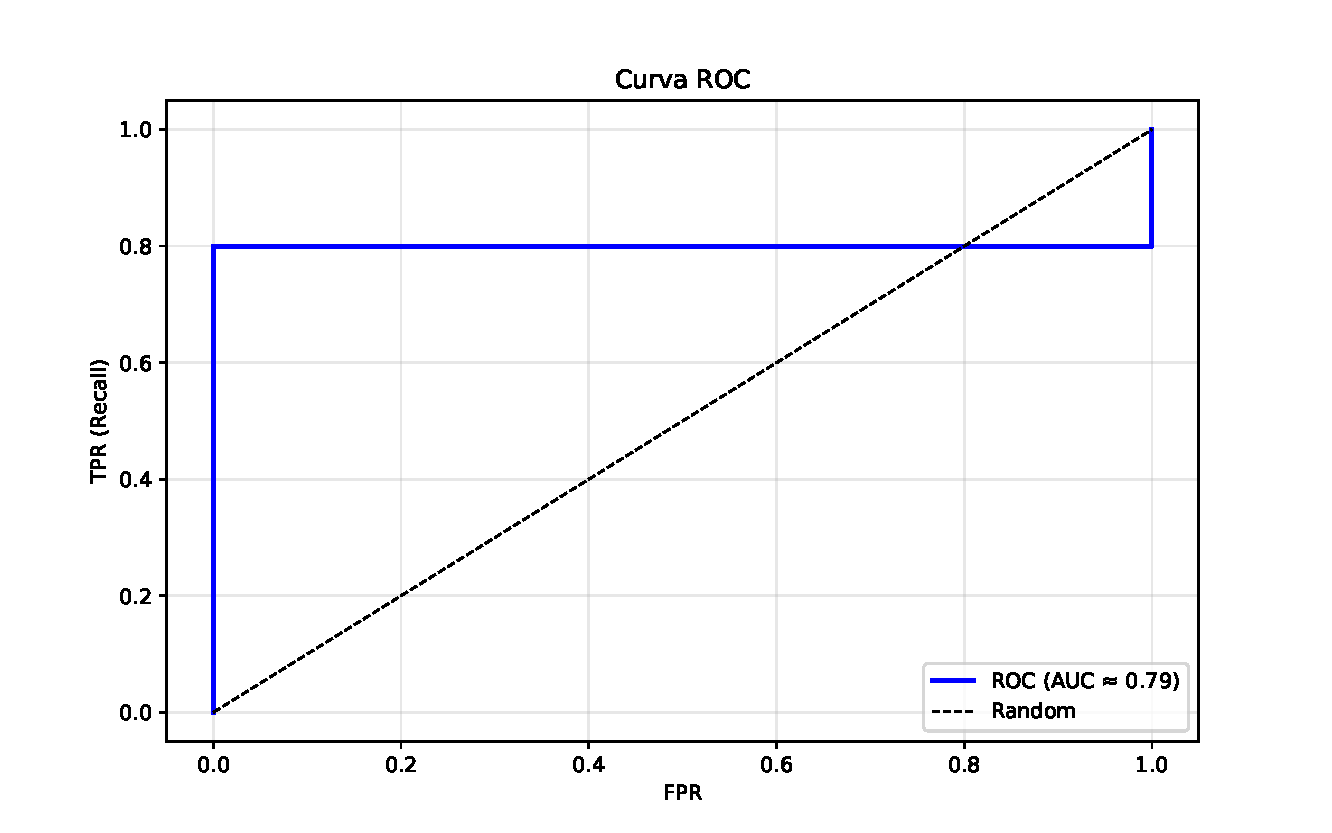
\includegraphics[width=0.85\textwidth]{LSTM/roc.pdf}
      \caption{Curva ROC y AUC del LSTM Autoencoder}
      \label{fig:roc_lstm}
\end{figure}

El resultado principal del proceso de validación se puede observar directamente en el siguiente gráfico, que muestra el momento exacto en que el modelo detecta una anomalía.

\begin{figure}[ht!]
      \centering
      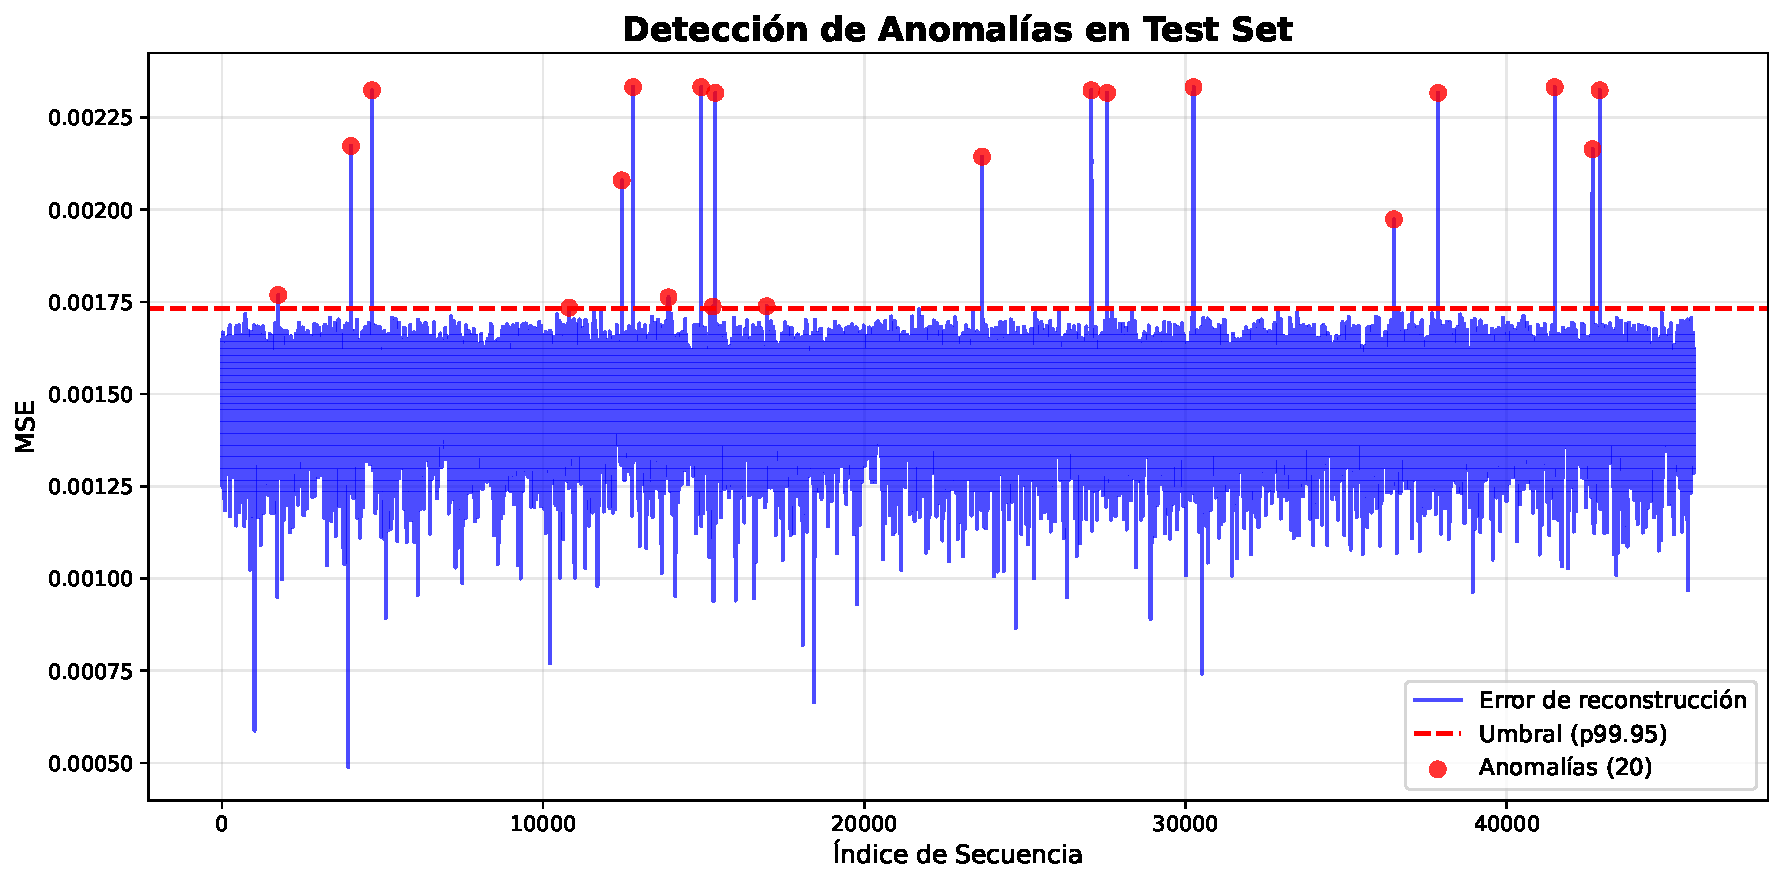
\includegraphics[width=0.85\textwidth]{LSTM/anomalias.pdf}
      \caption{Gráficas de MSE por secuencia para el LSTM Autoencoder.}
      \label{fig:mse_lstm}
\end{figure}

En la gráfica de la figura \ref{fig:mse_lstm}, se visualiza el error de reconstrucción para cada secuencia del conjunto de prueba. La línea discontinua roja representa el umbral de anomalía (MSE = 0.001646). Los puntos rojos marcan las 21 secuencias cuyo error superó este límite, siendo clasificadas correctamente como anomalías. Este gráfico confirma visualmente que el modelo es efectivo para asignar una puntuación de error mucho más alta a los eventos que se desvían del comportamiento normal aprendido.

Para analizar en detalle el rendimiento del modelo, no es suficiente con saber el número total de anomalías detectadas. Es fundamental comprender la naturaleza de sus aciertos y errores, y para ello se utiliza la matriz de confusión. Esta herramienta es una tabla que desglosa los resultados al comparar las predicciones del modelo con la realidad del conjunto de prueba, permitiéndonos visualizar cuatro escenarios clave:

\begin{itemize}
      \item Verdaderos Positivos (VP): Las anomalías que el modelo identificó correctamente.
      \item Verdaderos Negativos (VN): Los eventos normales que el modelo clasificó correctamente como normales.
      \item Falsos Positivos (FP): Eventos normales que el modelo etiquetó erróneamente como anomalías (las ``falsas alarmas'').
      \item Falsos Negativos (FN): Las anomalías reales que el modelo no fue capaz de detectar (los errores más críticos).
\end{itemize}

\begin{table}[ht!]
      \doublespacing
      \small
      \centering
      \begin{tabular}{ >{\centering\arraybackslash}p{3cm} >{\centering\arraybackslash}p{3cm} >{\centering\arraybackslash}p{3cm} }
            \hline
                          & \multicolumn{2}{c}{\textbf{Esperado}}              \\
            \hline
            \textbf{Real} & \textbf{P}                            & \textbf{N} \\
            \hline
            V             & 18                                    & 6      \\
            F             & 3                                     & 45814          \\
            \hline
      \end{tabular}
      \caption{Matriz de Confusión del LSTM Autoencoder}
      \label{tab:confusion_matrix_lstm}
\end{table}

VP (Verdaderos Positivos): 18

FP (Falsos Positivos): 3

FN (Falsos Negativos): 6

VN (Verdaderos Negativos): 45814

Estas cifras se traducen en las siguientes métricas de rendimiento:

\begin{itemize}
      \item  Exactitud (Accuracy): proporción de predicciones correctas respecto al total de casos evaluados.

            \begin{align}
                  Accuracy = \frac{TP+TN}{TP+TN+FP+FN}=\frac{(18+45814)}{(18+45814+3+6)}\approx 0.9998 \notag \\
                  \label{eq:accuracy}
            \end{align}
            \myequations{Accuracy para LSTM Autoencoder}


      \item Tasa de error: proporción de predicciones incorrectas respecto al total.

            \begin{align}
                  Error = \frac{FP+FN}{TP+TN+FP+FN}=\frac{(3+6)}{(18+45814+3+6)}\approx 0.0002 \notag \\
                  \label{eq:error}
            \end{align}
            \myequations{Tasa de Error para LSTM Autoencoder}

      \item Sensibilidad (Recall o Verdaderos Positivos): proporción de eventos de anomalos correctamente detectados.

            \begin{align}
                  Recall = \frac{TP}{TP+FN} \notag \\
                  \label{eq:recall}
            \end{align}
            \myequations{Recall para LSTM Autoencoder}

      \item Precisión: La proporción de casos realmente positivos entre todos los casos que el modelo predijo como positivos.

            \begin{align}
                  Precision = \frac{TP}{TP+FP}=\frac{18}{18+3}\approx 0.8571 \notag \\
                  \label{eq:precision}
            \end{align}
            \myequations{Precision para LSTM Autoencoder}

      \item Especificidad: proporción de eventos no críticos correctamente descartados.

            \begin{align}
                  Specificity = \frac{TN}{TN+FP}=\frac{45814}{45814+3}\approx 0.9999 \notag \\
                  \label{eq:specificity}
            \end{align}
            \myequations{Specificity para LSTM Autoencoder}

      \item F1 Score: media armónica entre la precisión y la sensibilidad, útil cuando es importante equilibrar ambas.

            \begin{align}
                  F1_{score} = 2 \cdot \frac{Precision \cdot Recall}{Precision + Recall} = 2 \cdot \frac{0.8571 * 0.75}{0.8571+0.75} \approx 0.8 \notag \\
                  \label{eq:f1score}
            \end{align}
            \myequations{F1 Score para LSTM Autoencoder}

\end{itemize}

El análisis de las métricas de rendimiento cuantifica el desempeño del modelo. La exactitud general es del 99.98\%, aunque este valor es menos indicativo en conjuntos de datos con clases desbalanceadas. Un análisis más específico muestra una Sensibilidad (Recall) del 75.0\%, lo que indica que el modelo identifica a tres de cada cuatro anomalías reales. A su vez, la Precisión es del 85.7\%, lo que significa que sus alertas positivas son correctas en esa proporción. La puntuación F1, como media armónica de ambas, se sitúa en 80.0\%, reflejando el balance entre la capacidad de detección y la fiabilidad de sus predicciones.

Por último, la curva ROC (figura \ref{fig:roc_lstm}) y su AUC de 0.792 confirman que el modelo tiene una buena capacidad para distinguir entre comportamientos normales y anómalos, situándose cerca del umbral deseado de 0.8. En conjunto, estos resultados validan la efectividad del LSTM Autoencoder para la detección de anomalías en secuencias de eventos en nuestro contexto específico.

\uparagraph{Evaluacion del Isolation Forest}

Para la  evaluación del modelo Isolation Forest (IF), una técnica no supervisada que opera de manera fundamentalmente distinta al autoencoder. En lugar de medir un error de reconstrucción, este modelo asigna una ``puntuación de anomalía'' a cada evento basándose en qué tan fácil es aislarlo del resto de los datos. Los eventos que son más fáciles de separar (requieren menos divisiones en los árboles de decisión) se consideran más anómalos.

Funciona construyendo múltiples árboles de decisión (en este caso, 100) estos arboles se construyen al dividir aleatoriamente los datos en subconjuntos. Funciona bajo la premisa de que las anomalías son puntos de datos que se encuentran en regiones menos densas del espacio de características, por lo que son más fáciles de aislar. Cada evento recibe una puntuación basada en la profundidad promedio a la que aparece en los árboles; cuanto más cerca esté la puntuación de 1, más anómalo es el evento.

El proceso de evaluación se aplicó sobre el mismo conjunto de datos, compuesto por 100,809 registros, de los cuales 5,041 (5\%) son anomalías reales. A diferencia del LSTM Autoencoder, el umbral de decisión en el Isolation Forest no se calcula estadísticamente a posteriori, sino que se define a priori mediante el hiperparámetro contamination. Este valor se estableció en 0.05 (5\%), una práctica estándar para configurar este algoritmo. Cualquier evento cuya puntuación de anomalía superara el umbral derivado de esta configuración fue clasificado como anómalo.

\begin{figure}[ht!]
      \centering
      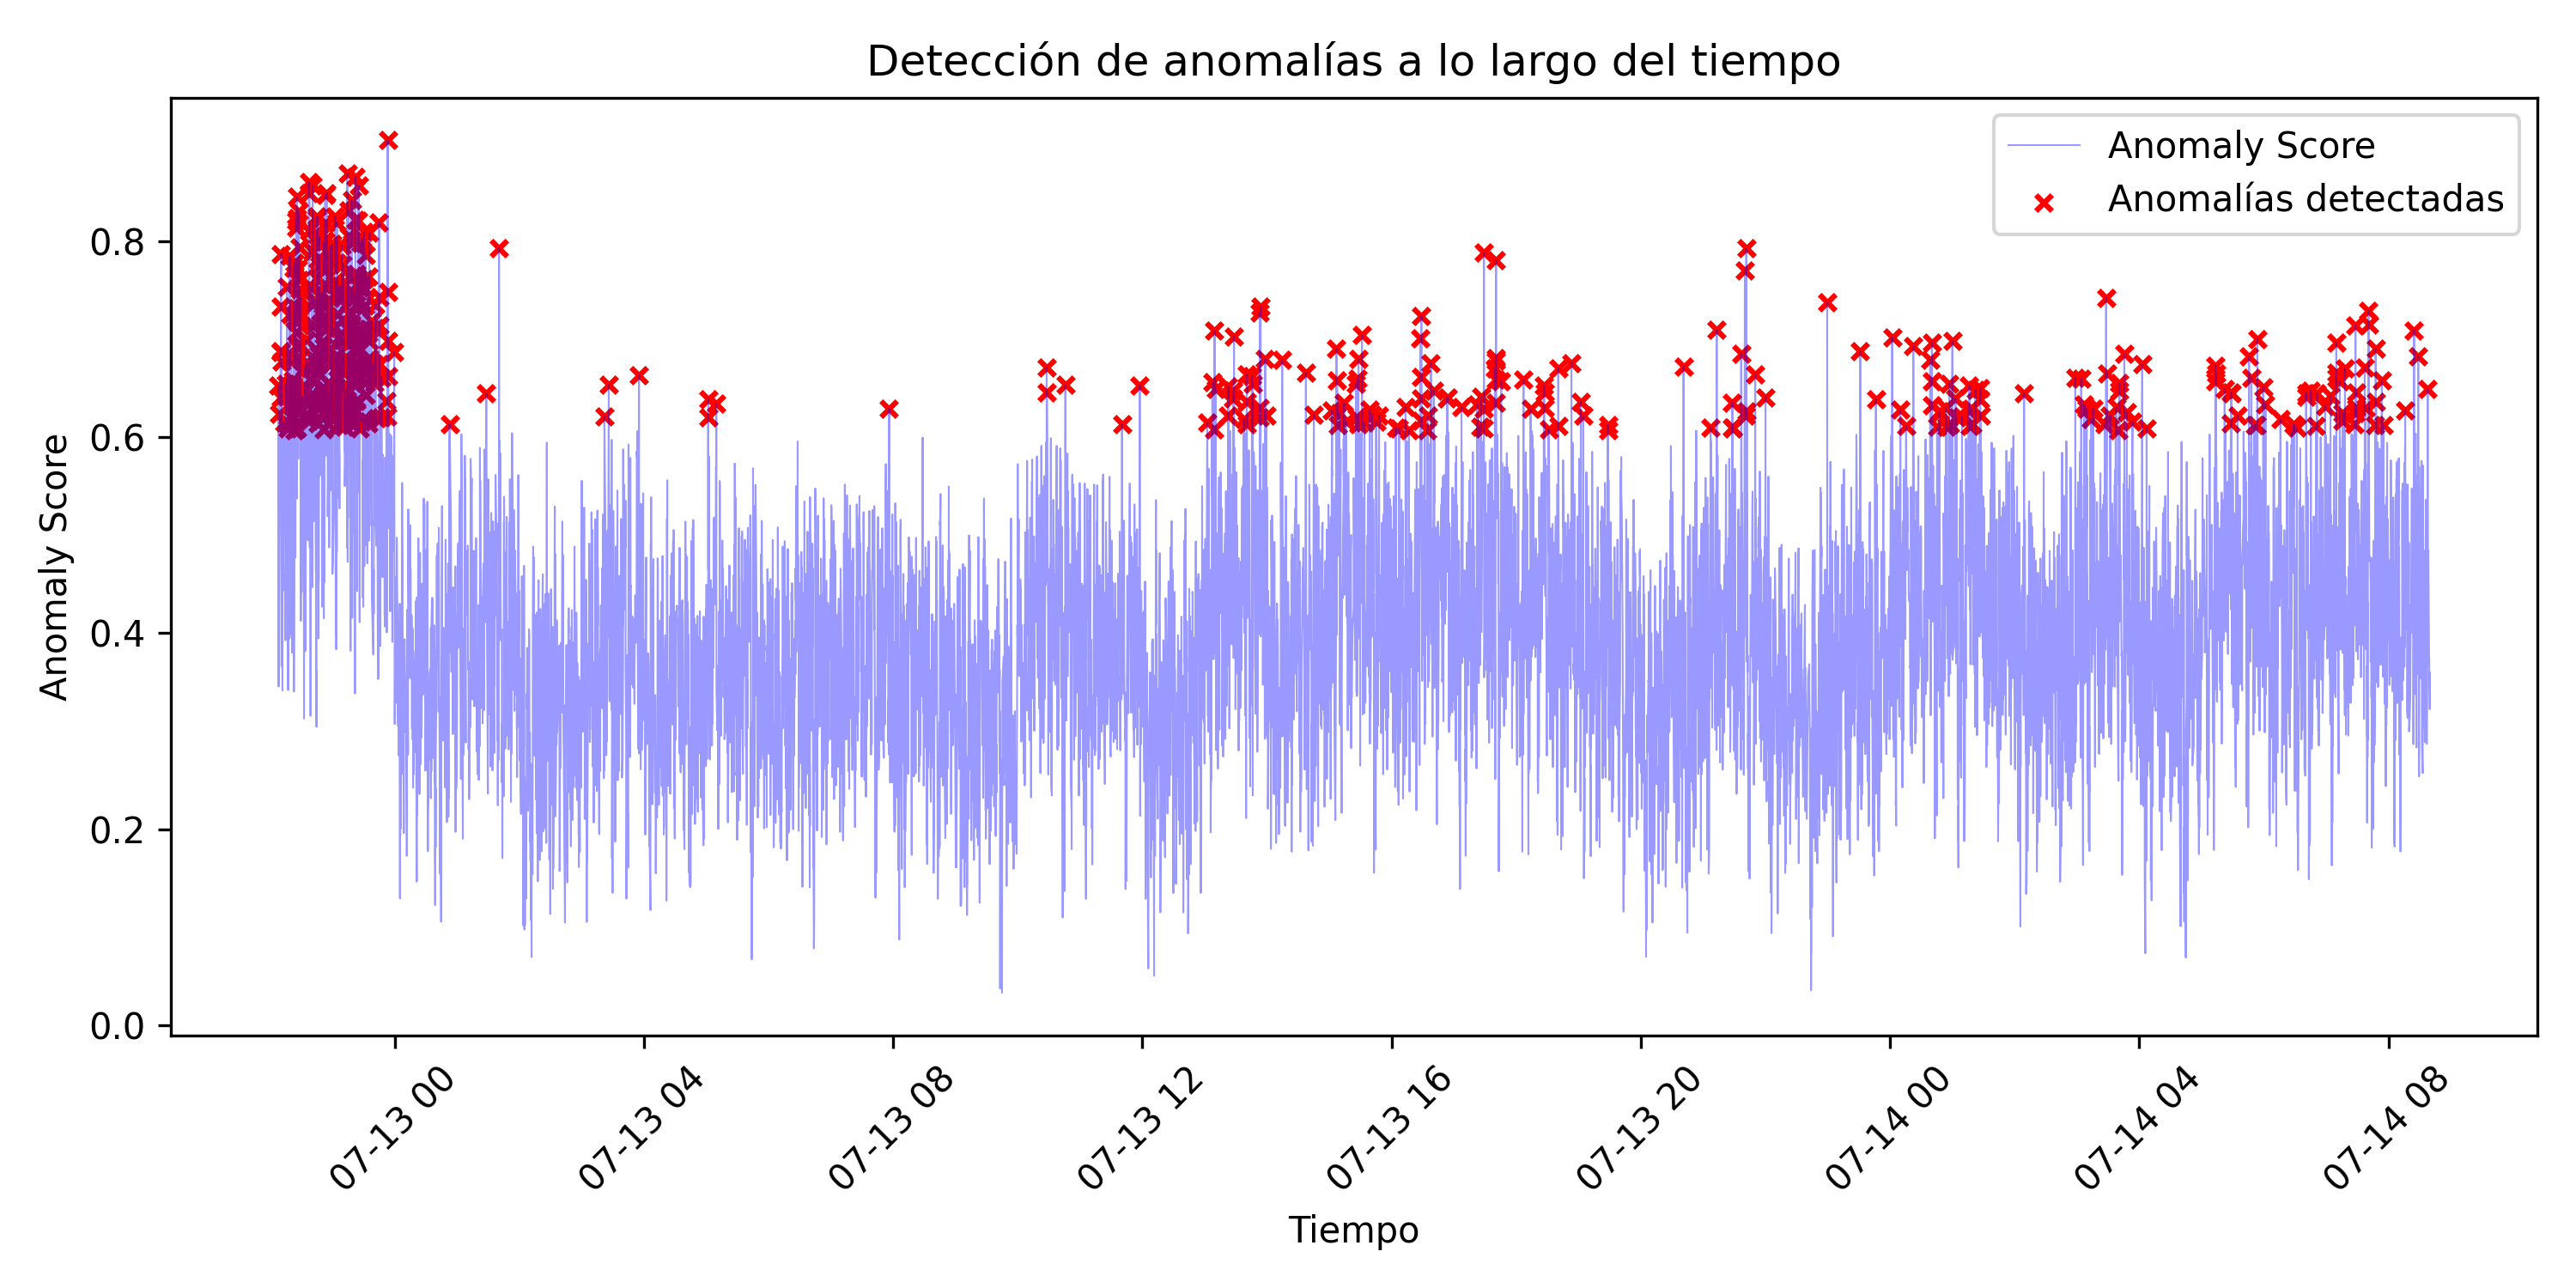
\includegraphics[width=0.85\textwidth]{IF/anomalias_tiempo.png}
      \caption{Gráficas de puntuación de anomalía por evento para el Isolation Forest.}
      \label{fig:anomalias_if}
\end{figure}

\begin{itemize}
      \item Análisis de la Detección

            El análisis de los resultados del Isolation Forest revela un rendimiento significativamente inferior al del LSTM Autoencoder. El modelo identificó un total de 5,041 eventos como anómalos. Sin embargo, un desglose más profundo a través de la matriz de confusión es necesario para entender la verdadera efectividad de estas detecciones.

            Para analizar en detalle el rendimiento del modelo, se utiliza la matriz de confusión. Esta herramienta desglosa los resultados al comparar las predicciones del modelo con la realidad del conjunto de prueba, permitiéndonos visualizar cuatro escenarios clave:

            \begin{table}[ht!]
                  \doublespacing
                  \small
                  \centering
                  \begin{tabular}{ >{\centering\arraybackslash}p{3cm} >{\centering\arraybackslash}p{3cm} >{\centering\arraybackslash}p{3cm} }
                        \hline
                                      & \multicolumn{2}{c}{\textbf{Esperado}}              \\
                        \hline
                        \textbf{Real} & \textbf{P}                            & \textbf{N} \\
                        \hline
                        V             & 2877                                  & 8031      \\
                        F             & 2164                                  & 87737       \\
                        \hline
                  \end{tabular}
                  \caption{Matriz de Confusión del Isolation Forest}
                  \label{tab:confusion_matrix_isolation_forest}
            \end{table}

            VP (Verdaderos Positivos): 2,877

            FP (Falsos Positivos): 2,164

            FN (Falsos Negativos): 8,031

            VN (Verdaderos Negativos): 87,737

            % \begin{figure}[ht!]
            %       \centering
            %       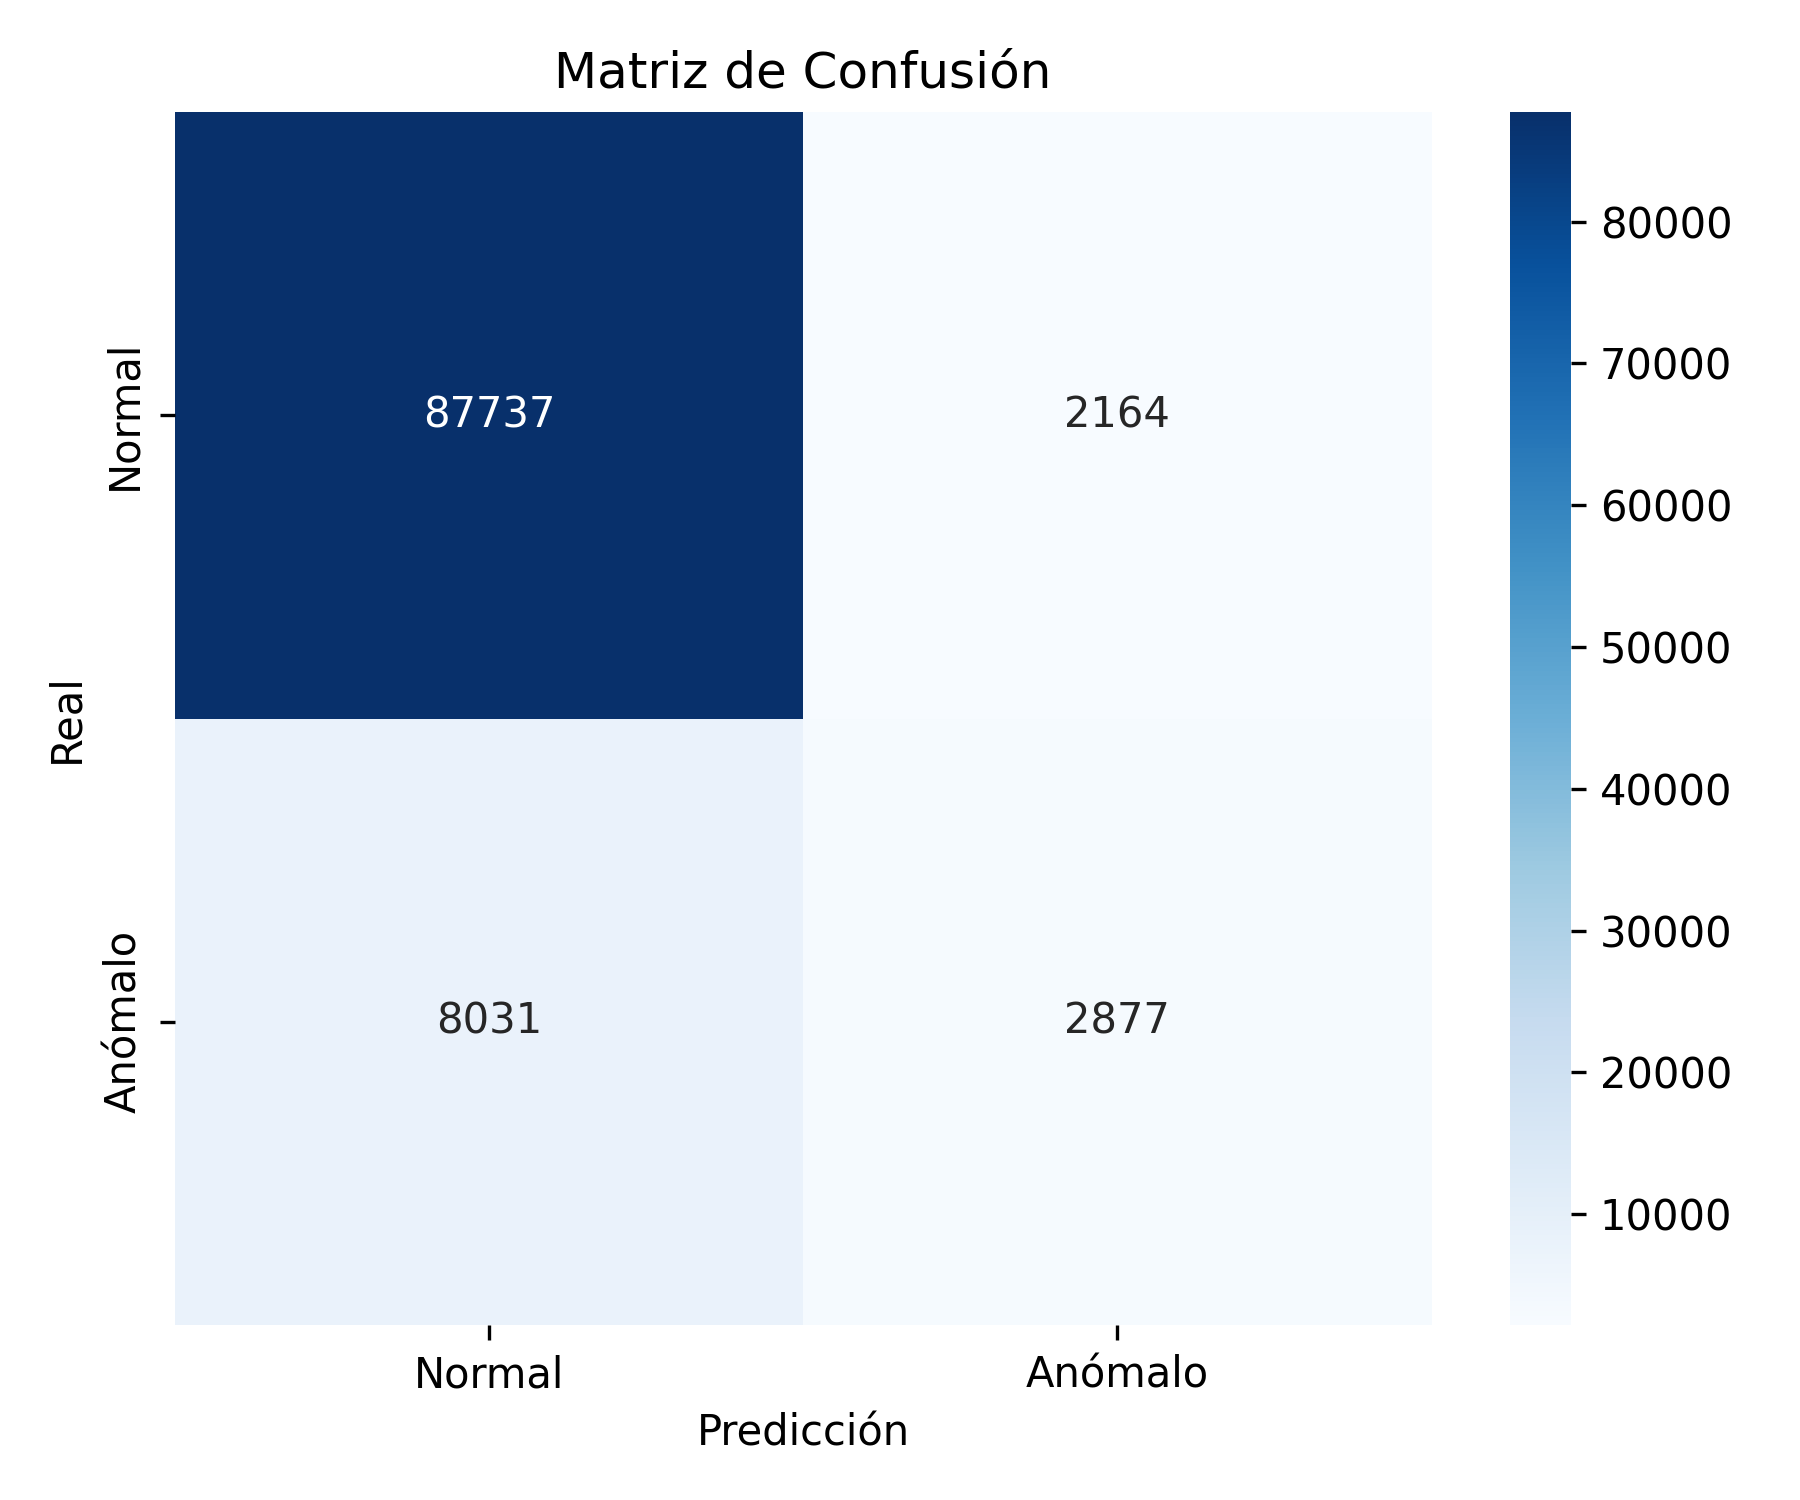
\includegraphics[width=0.65\textwidth]{IF/matriz_confusion.png}
            %       \caption{Matriz de Confusión del Isolation Forest}
            %       \label{fig:confusion_matrix_if}
            % \end{figure}

      \item Métricas de Rendimiento

            \begin{align}
                  Accuracy = \frac{(2877+87737)}{(2877+87737+2164+8031)}\approx 0.8989 \notag \\
                  \label{eq:accuracy_if}
            \end{align}
            \myequations{Accuracy para Isolation Forest}


            \begin{align}
                  Error = \frac{(2164+8031)}{(2877+87737+2164+8031)}\approx 0.101 \notag \\
                  \label{eq:error_if}
            \end{align}
            \myequations{Tasa de Error para Isolation Forest}

            \begin{align}
                  Recall = \frac{2877}{2877+8031}\approx 0.2638 \notag \\
                  \label{eq:recall_if}
            \end{align}
            \myequations{Recall para Isolation Forest}

            \begin{align}
                  Precision = \frac{2877}{2877+2164}\approx 0.5707 \notag \\
                  \label{eq:precision_if}
            \end{align}
            \myequations{Precision para Isolation Forest}

            \begin{align}
                  Specificity = \frac{87737}{87737+2164}\approx 0.9759 \notag \\
                  \label{eq:specificity_if}
            \end{align}
            \myequations{Specificity para Isolation Forest}

            \begin{align}
                  F1_{score} = 2 \cdot \frac{Precision * Recall}{Precision+Recall} \notag \\
                  \label{eq:f1_if}
            \end{align}
            \myequations{F1 Score para Isolation Forest}

\end{itemize}

\begin{figure}[ht!]
      \centering
      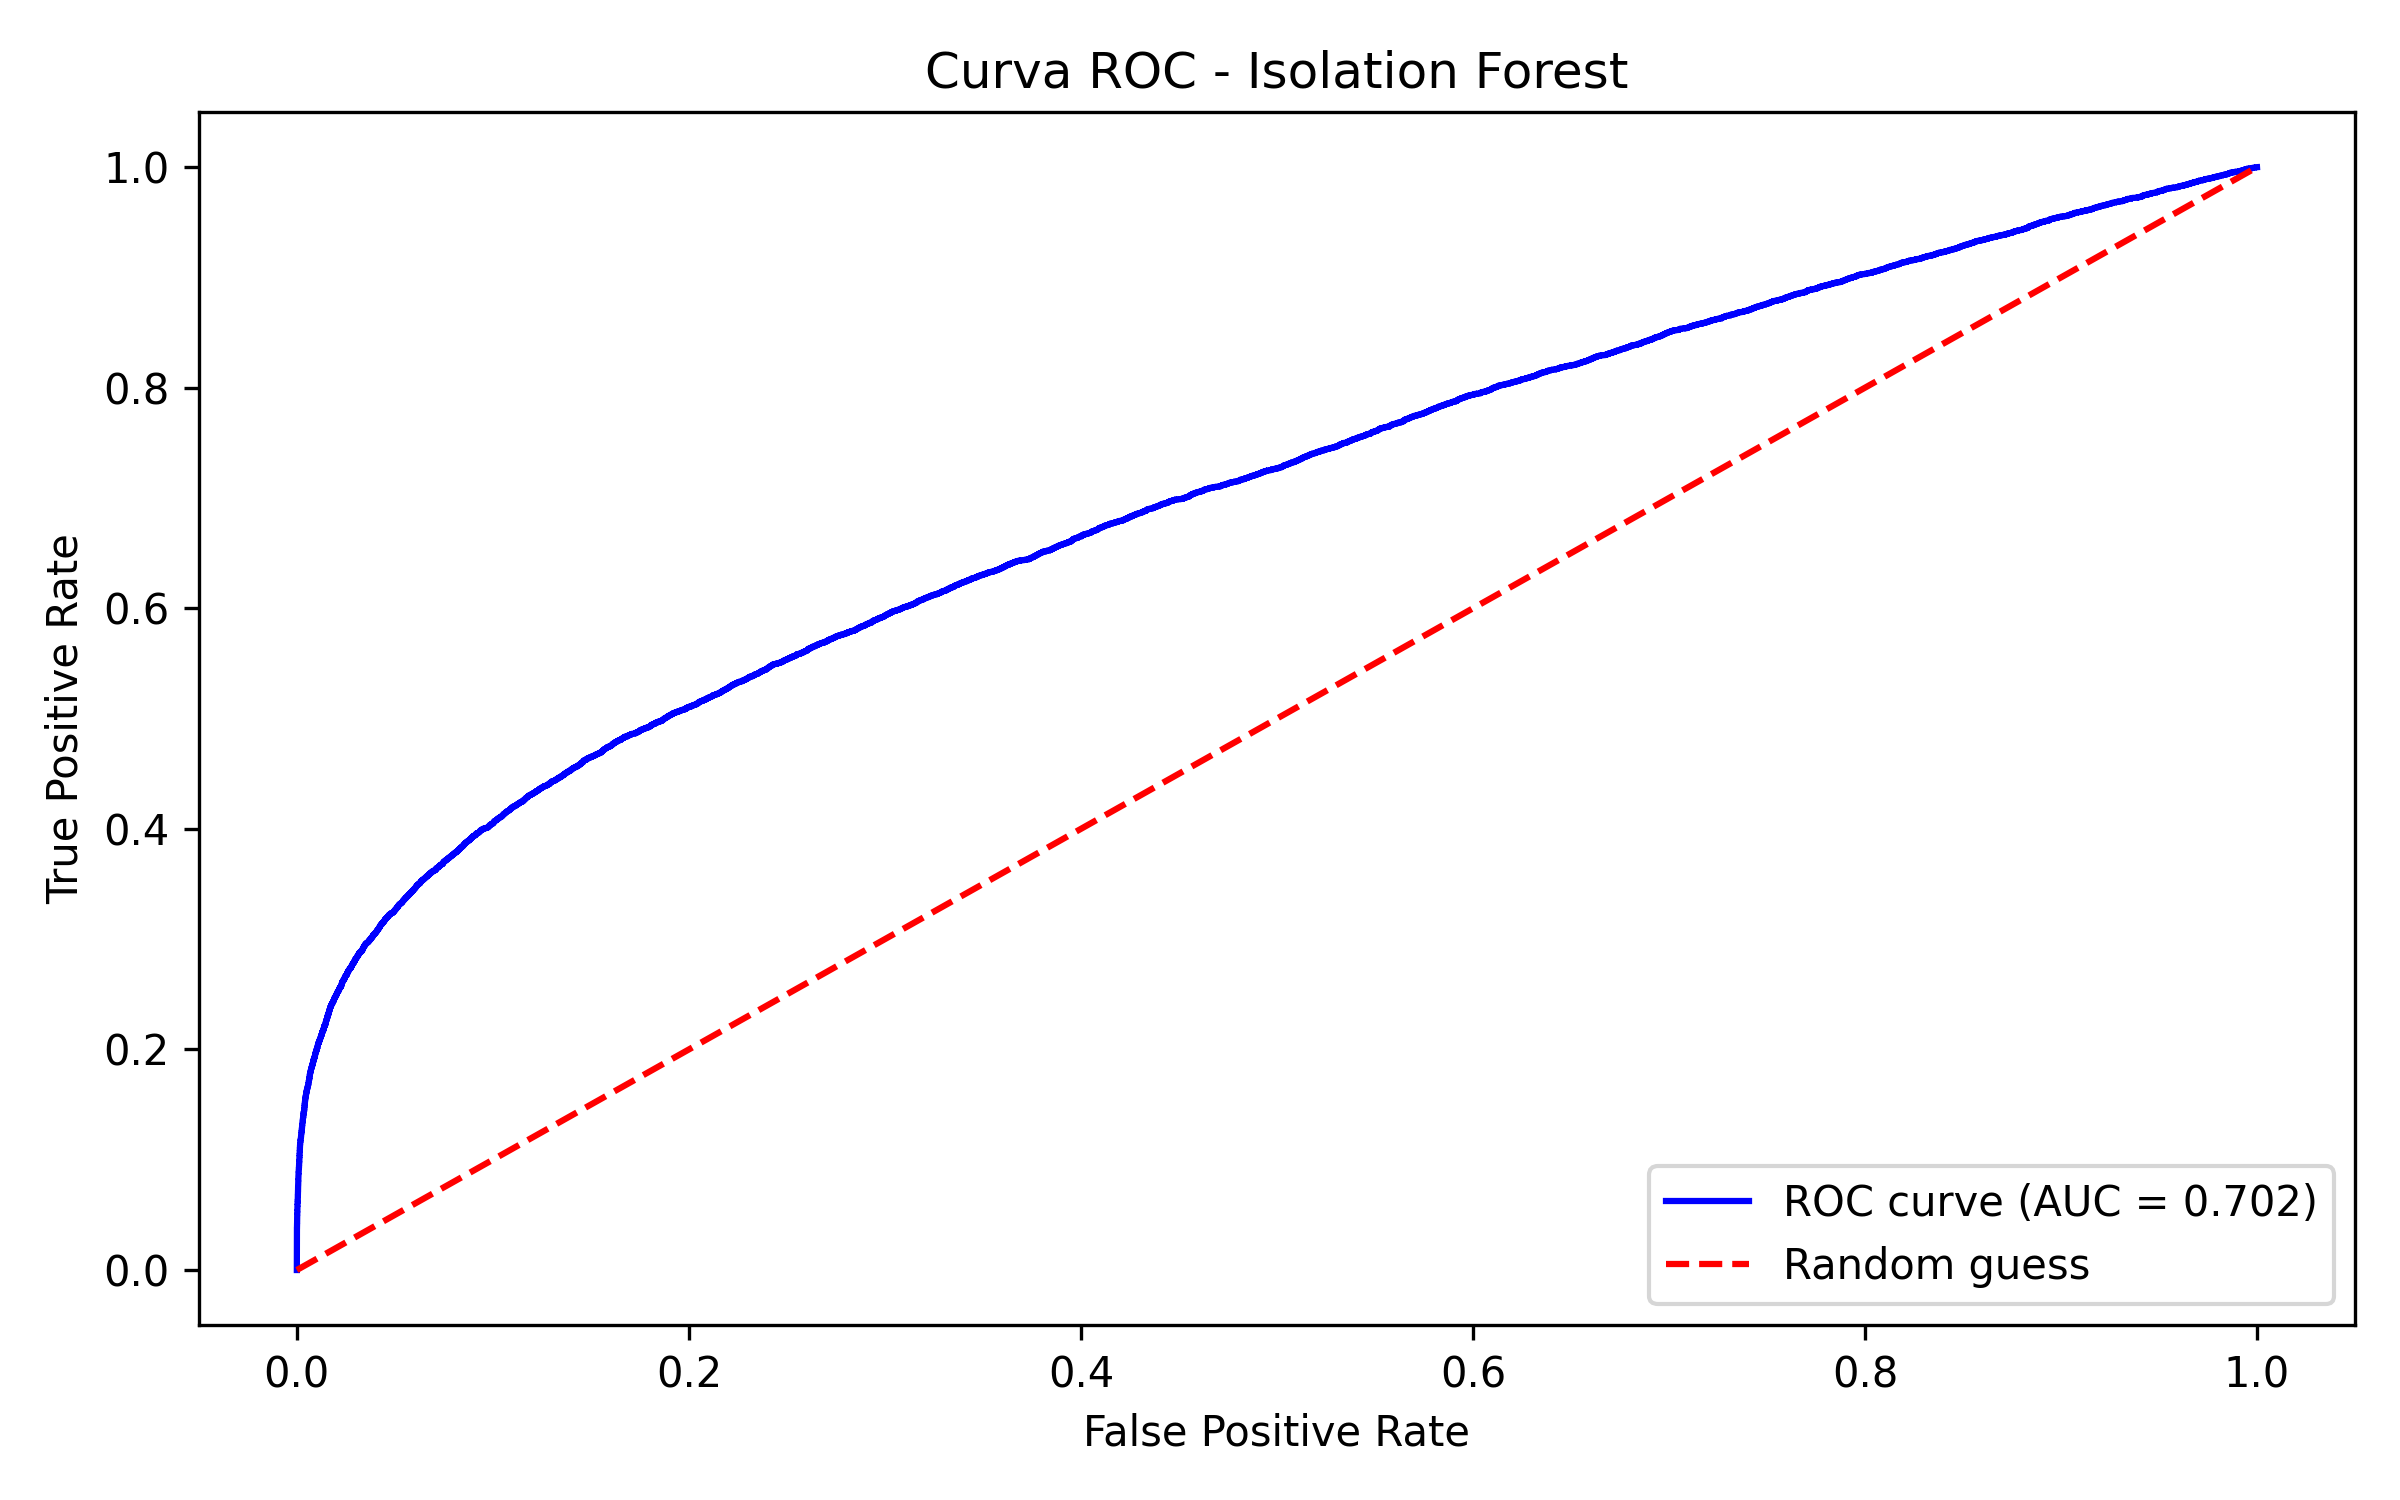
\includegraphics[width=0.85\textwidth]{IF/roc_auc.png}
      \caption{Curva ROC y AUC del Isolation Forest.}
      \label{fig:roc_if}
\end{figure}

El análisis de las métricas de rendimiento cuantifica el desempeño del modelo. La exactitud general del 89.9\% es un valor engañoso, inflado por la gran cantidad de eventos normales correctamente identificados. Las métricas más importantes revelan un rendimiento bajo: una Sensibilidad (Recall) de solo el 26.4\%, lo que indica que el modelo no detectó a más de 3 de cada 4 anomalías reales. A su vez, la Precisión es del 57.1\%, lo que significa que casi la mitad de sus alertas son falsas alarmas. La puntuación F1 resultante, del 36.1\%, confirma que el modelo, en su configuración actual, carece de la capacidad necesaria para una detección fiable de anomalías en este contexto.

La curva ROC (figura \ref{fig:roc_if}) y su AUC de 0.612 refuerzan esta conclusión, situando al modelo muy por debajo del umbral deseado de 0.8. En conjunto, estos resultados indican que el Isolation Forest, con los hiperparámetros adoptados, no es adecuado para la detección de anomalías en secuencias de eventos en nuestro contexto específico.

En la figura \ref{fig:anomalias_if}, se visualiza la puntuación de anomalía asignada por el modelo a cada evento del conjunto de prueba. Los puntos rojos marcan los eventos cuya puntuación superó este límite, siendo clasificados como anomalías. Este gráfico ilustra cómo el modelo asigna puntuaciones más altas a ciertos eventos, pero la distribución de estas puntuaciones no es lo suficientemente clara como para distinguir entre comportamientos normales y anómalos.


\usubsection{Sexta Iteración}
      En esta sexta iteración, luego de evaluar los resultados obtenidos con ambos modelos, se decidió adoptar el LSTM Autoencoder como solución principal para la detección de anomalías en el sistema de monitoreo acústico. Esta elección se fundamentó en su desempeño superior durante la fase de evaluación, donde superó significativamente al modelo Isolation Forest en todas las métricas clave.

      Sin embargo, se identificó un riesgo técnico relevante: los hiperparámetros del LSTM Autoencoder fueron adoptados directamente del estudio de \citeauthor{reis2025edge} \citeyear{reis2025edge}, sin una adaptación específica para nuestro conjunto de datos. Esto implica que, aunque el modelo mostró un rendimiento sólido, existe la posibilidad de que ajustes finos en estos parámetros puedan mejorar aún más su eficacia en nuestro contexto particular.
       \begin{figure}[ht!]
            \centering
            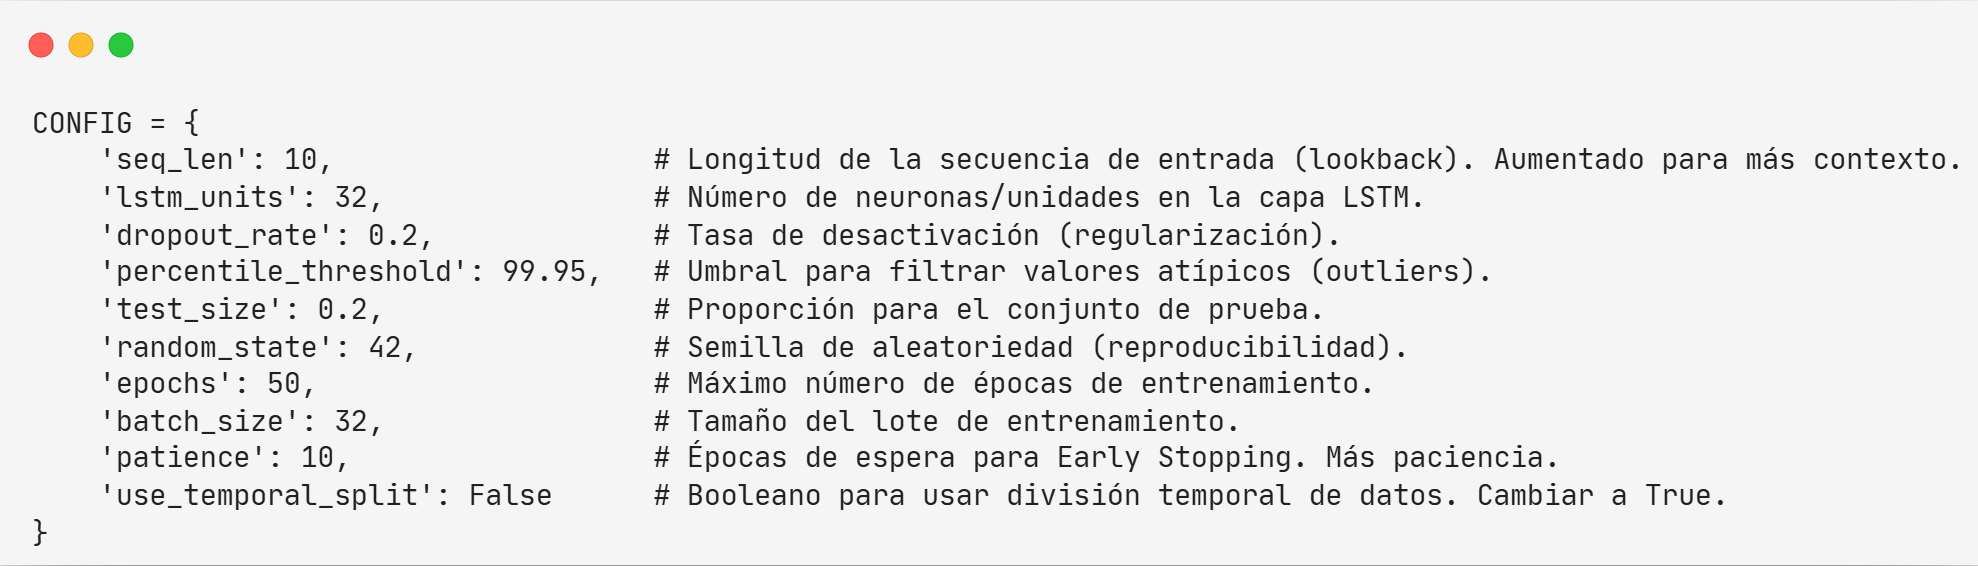
\includegraphics[width=0.85\textwidth]{Apendices/hiper_original.png}
            \caption{Parametros originales.}
            \label{fig:parametros_originales}
      \end{figure}

      Estos parametros se visualizan en la figura \ref{fig:parametros_originales}.

      Reconociendo esta limitación, se revisaron estudios sobre optimización de hiperparámetros, lo que derivó en la implementación de un proceso basado en optimización bayesiana. Esta técnica permitió mejorar los resultados obtenidos inicialmente, al encontrar mejores configuraciones más con menos evaluaciones del modelo.

      La optimización bayesiana, como se describe en el trabajo de \citeauthor{gardner2014bayesian} \citeyear{gardner2014bayesian}, utiliza modelos probabilísticos (usualmente procesos gaussianos) para estimar el comportamiento de la función objetivo y seleccionar los puntos de evaluación mediante funciones de adquisición que balancean exploración y explotación. Este enfoque es especialmente útil cuando tanto la función objetivo como las restricciones son costosas de evaluar, como ocurre en nuestro sistema de monitoreo acústico.

      Luego de aplicar este proceso de optimización, se obtuvieron nuevos valores para los hiperparámetros del LSTM Autoencoder, los cuales se detallan a continuación:

      \begin{figure}
            \centering
            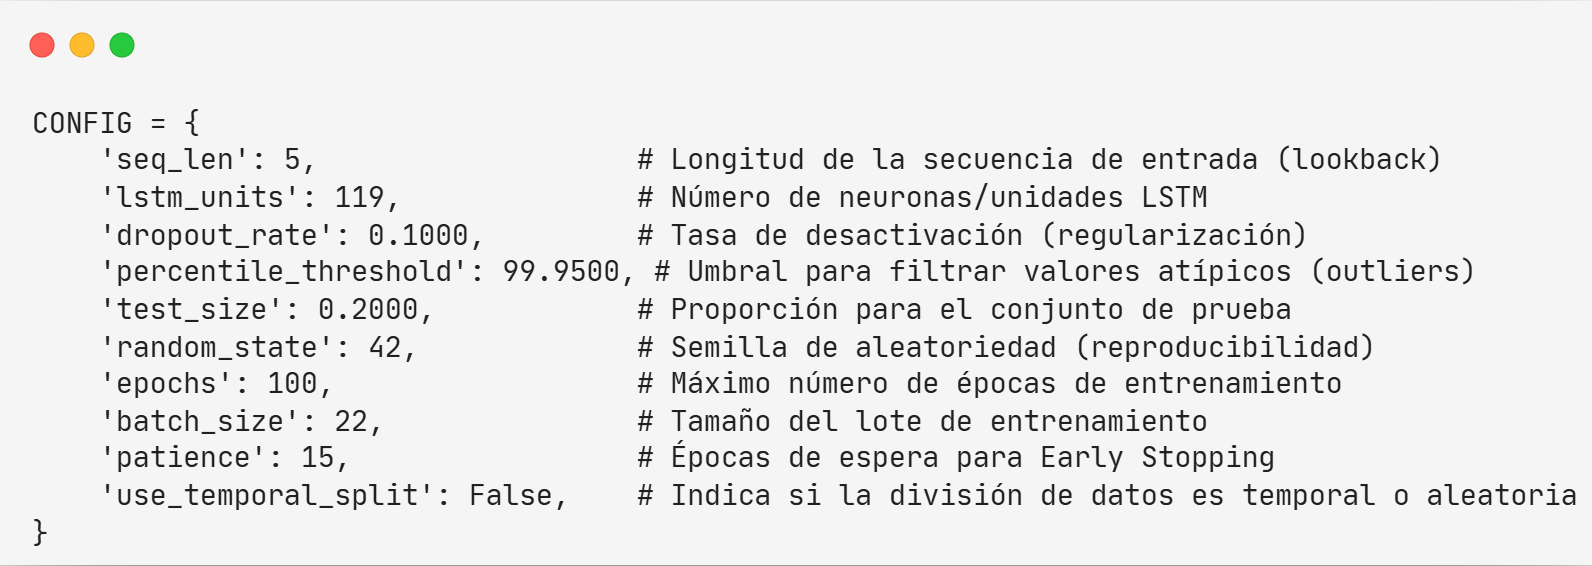
\includegraphics[width=0.85\textwidth]{Apendices/hiper_optimized.png}
            \caption{Parametros nuevos.}
            \label{fig:parametros_nuevos}
      \end{figure}


\usubsubsection{Evaluacion  del LSTM Autoencoder V2}

      Para evaluar el rendimiento del modelo  V2, se empleó el mismo conjunto de datos de prueba utilizado anteriormente, asegurando así una comparación directa y objetiva. Este conjunto contenía tanto secuencias de comportamiento normal como una serie de anomalías introducidas artificialmente para simular eventos atípicos.

      El proceso de evaluacion fue idéntico al aplicado previamente, pasando cada una de las 45,841 secuencias de prueba a través del autoencoder V2 y calculando su error de reconstrucción (MSE). Posteriormente, este error fue comparado con un umbral de anomalía redefinido tras la optimización bayesiana. Cualquier secuencia cuyo error de reconstrucción superara este nuevo umbral fue clasificada como una anomalía.

      \begin{figure}[ht!]
            \centering
            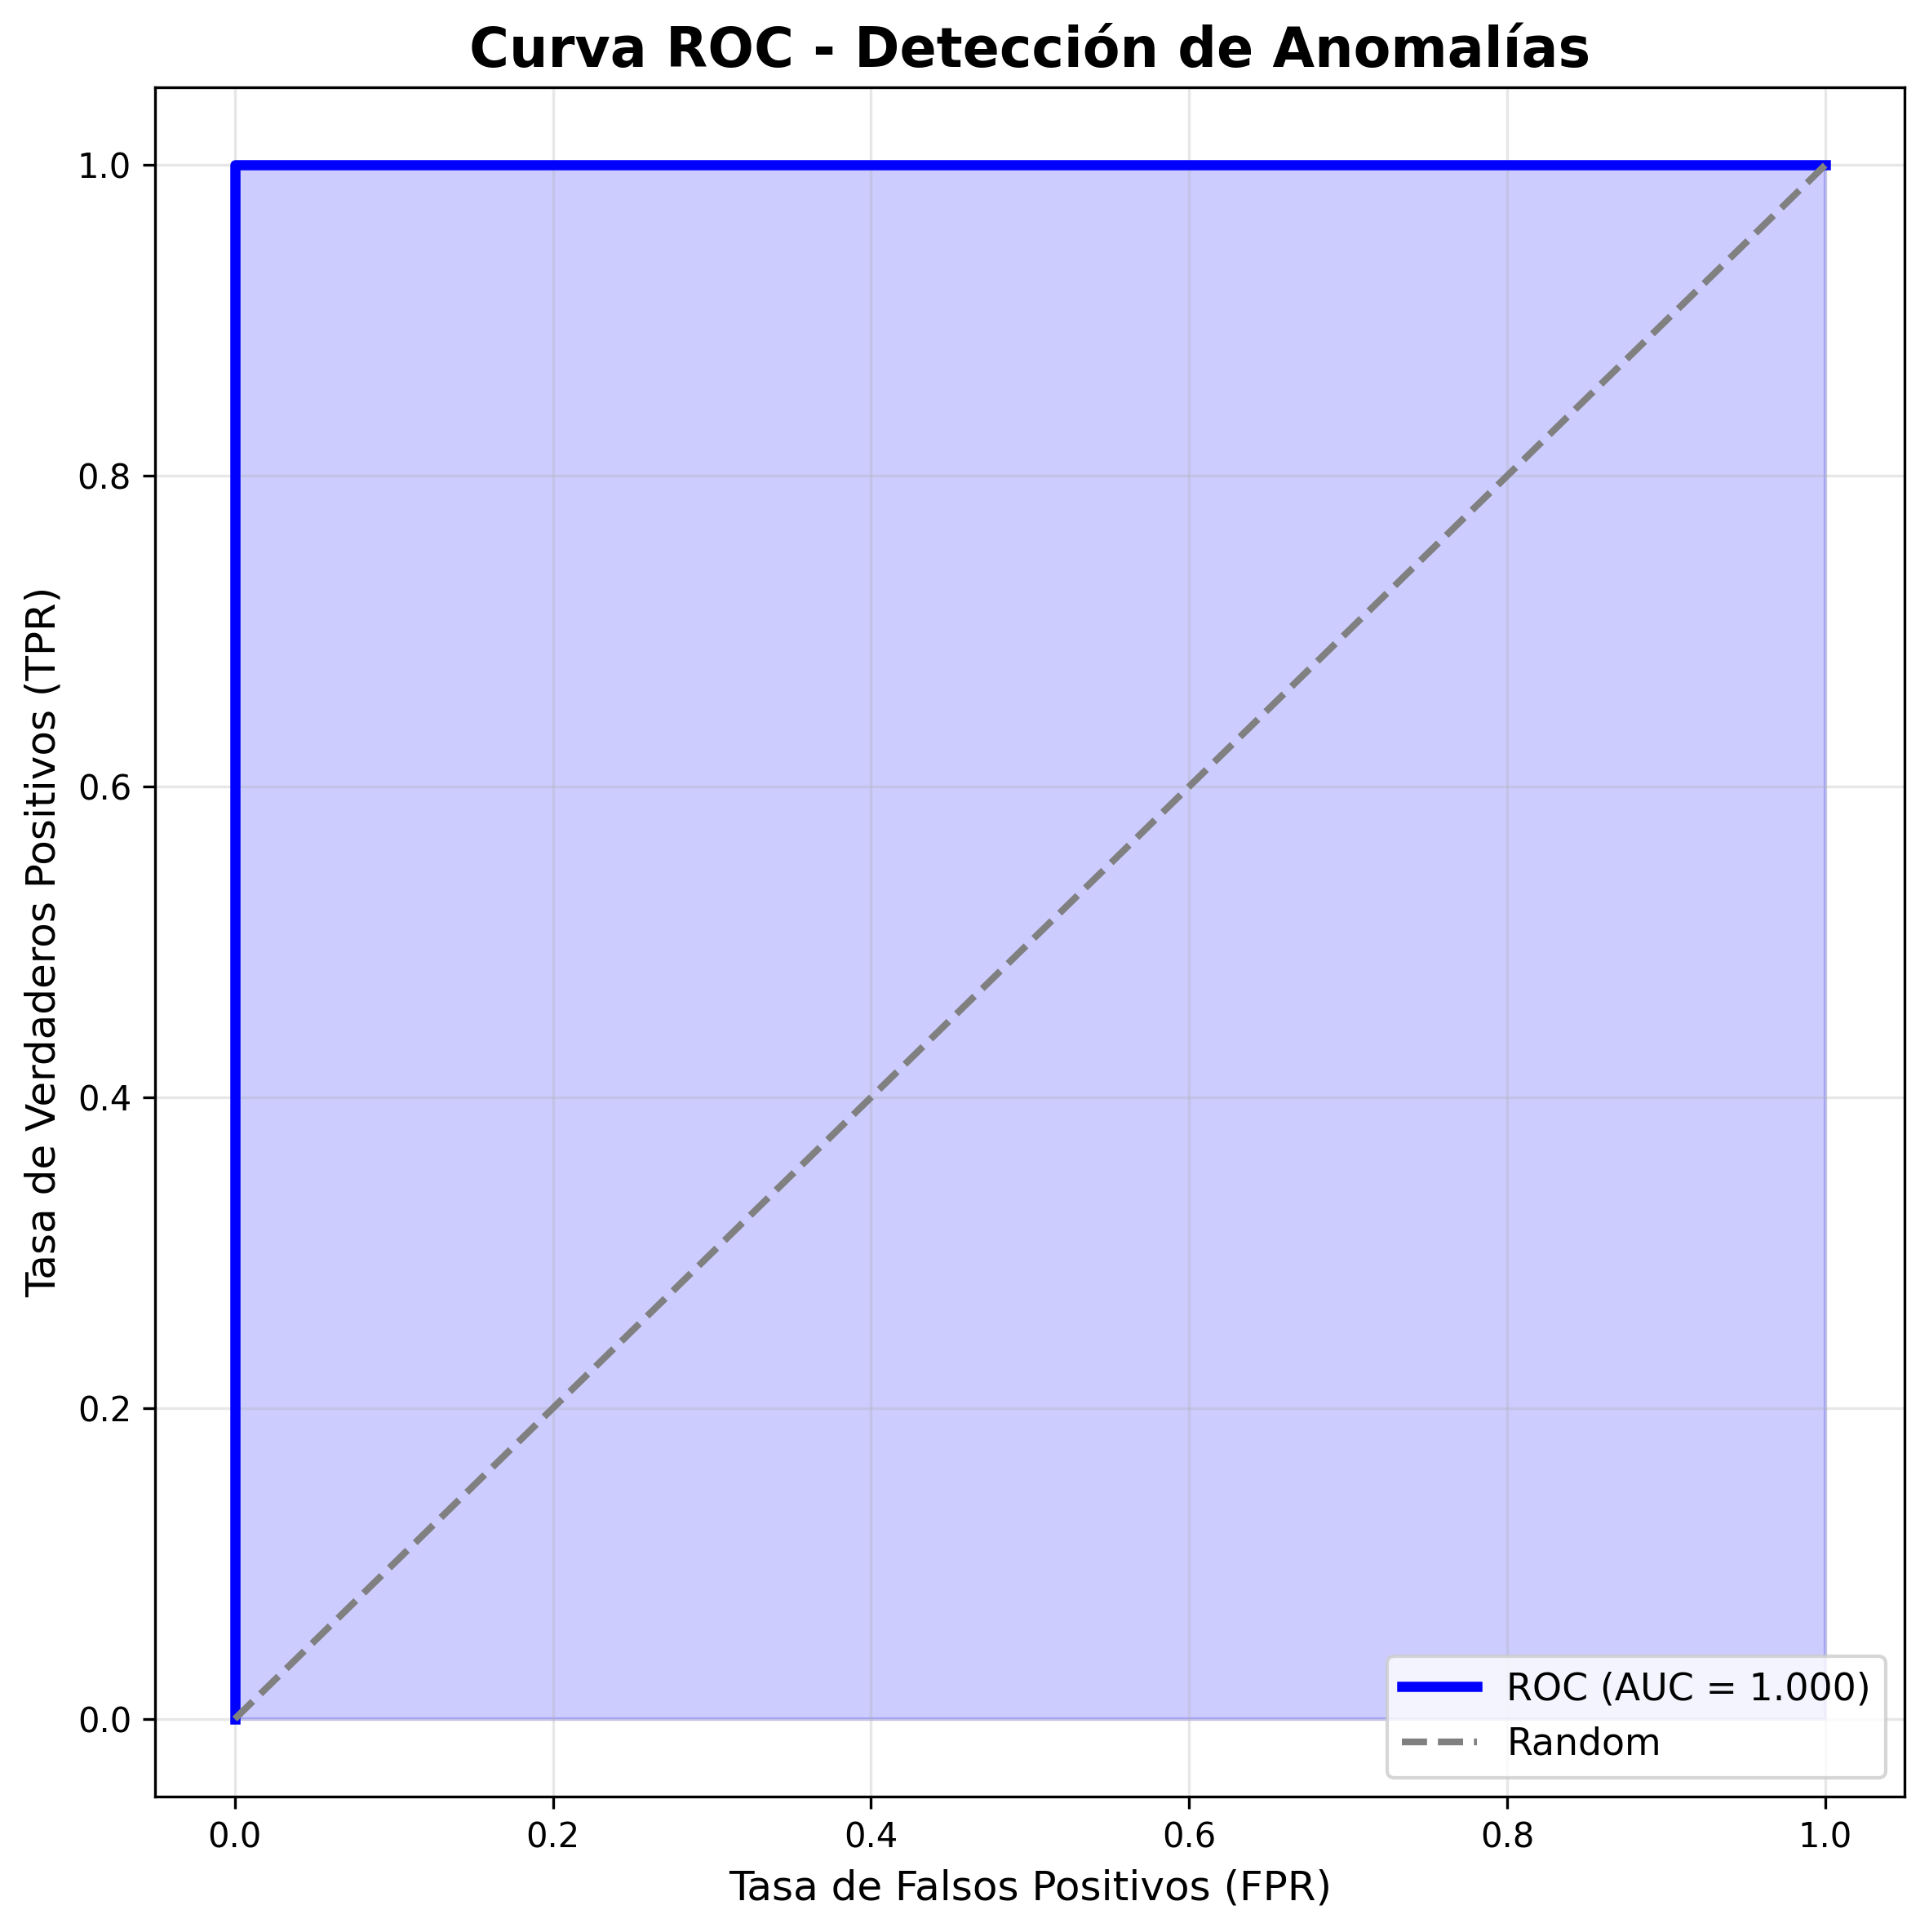
\includegraphics[width=0.85\textwidth]{LSTM/roc_optimized.png}
            \caption{Curva ROC y AUC del LSTM Autoencoder V2.}
            \label{fig:roc_lstm_optimized}
      \end{figure}

      \begin{figure}[ht!]
            \centering
            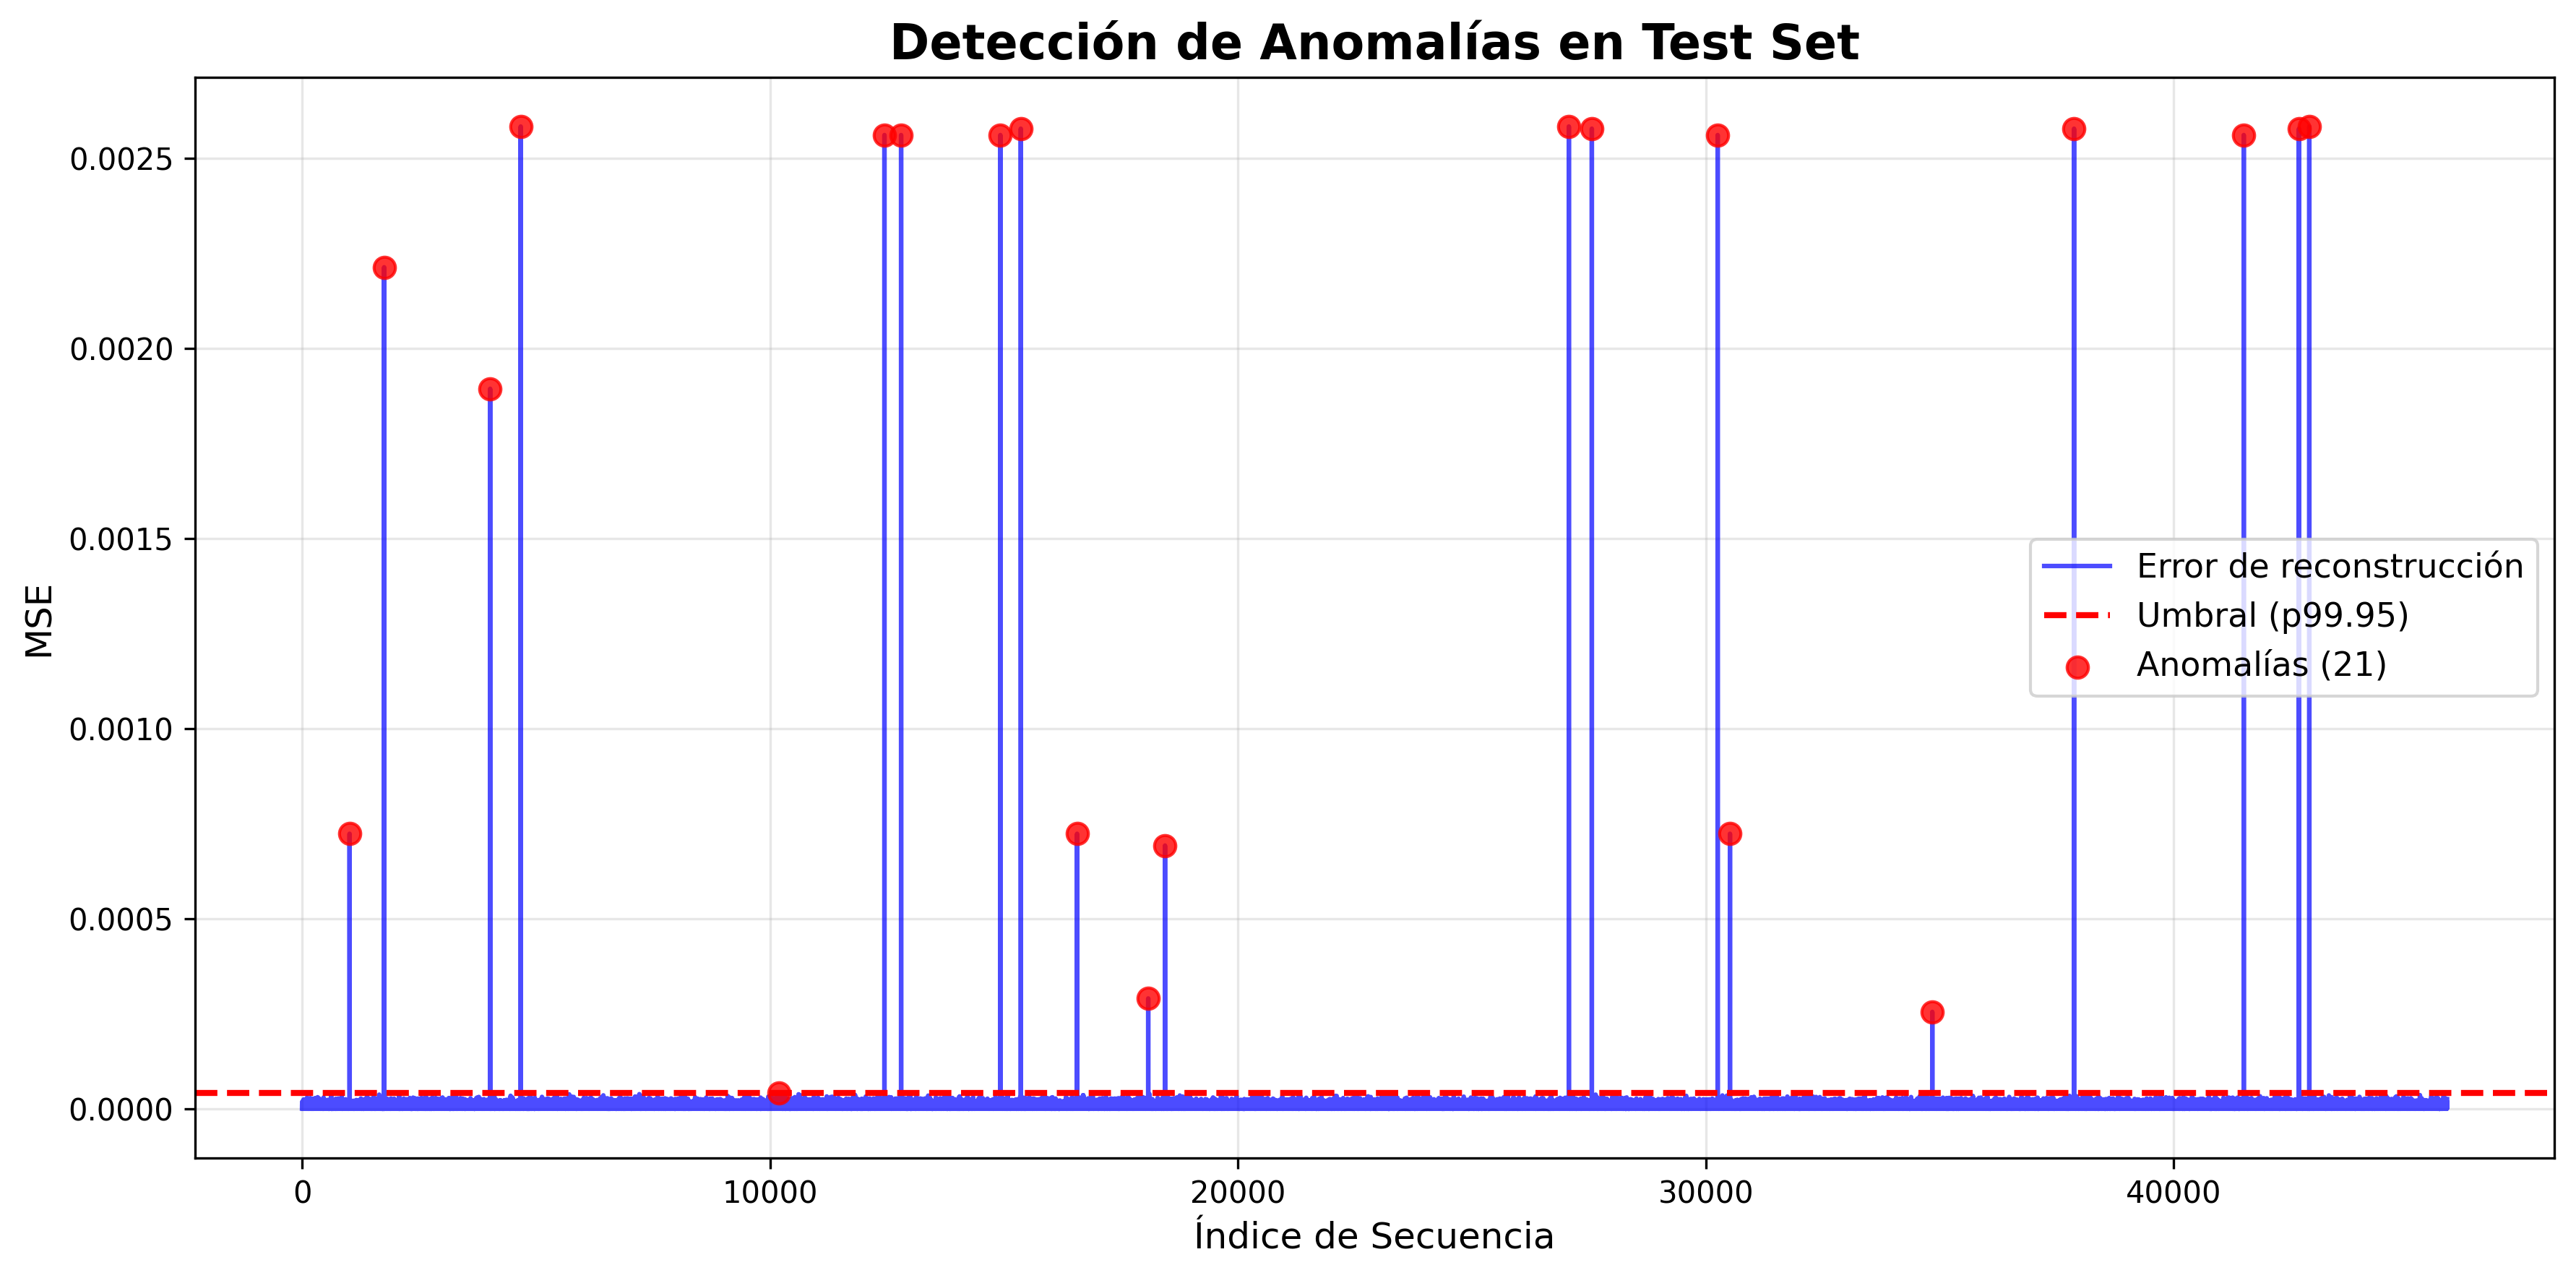
\includegraphics[width=0.85\textwidth]{LSTM/animalias_optimized.png}
            \caption{Gráficas de MSE por secuencia para el LSTM Autoencoder V2.}
            \label{fig:mse_lstm_optimized}
      \end{figure}

      En la gráfica de la figura \ref{fig:mse_lstm_optimized}, se visualiza el error de reconstrucción para cada secuencia del conjunto de prueba tras la optimización. La línea discontinua roja representa el nuevo umbral de anomalía. Los puntos rojos marcan las secuencias cuyo error superó este límite, siendo clasificadas correctamente como anomalías. Este gráfico confirma visualmente que el modelo optimizado es aún más efectivo para asignar una puntuación de error alta a los eventos que se desvían del comportamiento normal aprendido.

      \begin{table}[ht!]
            \doublespacing
            \small
            \centering
            \begin{tabular}{ >{\centering\arraybackslash}p{3cm} >{\centering\arraybackslash}p{3cm} >{\centering\arraybackslash}p{3cm} }
                  \hline
                                & \multicolumn{2}{c}{\textbf{Esperado}}              \\
                  \hline
                  \textbf{Real} & \textbf{P}                            & \textbf{N} \\
                  \hline
                  V             & 19                                    & 0  \\
                  F             & 2                                     & 45820         \\
                  \hline
            \end{tabular}
            \caption{Matriz de Confusión del LSTM Autoencoder V2}
            \label{tab:confusion_matrix_lstm_optimized}
      \end{table}

      VP (Verdaderos Positivos): 19
      FP (Falsos Positivos): 2
      FN (Falsos Negativos): 0
      VN (Verdaderos Negativos): 45820
      Estas cifras se traducen en las siguientes métricas de rendimiento:

      \begin{itemize}
            \item  Exactitud (Accuracy):

                  \begin{align}
                        Accuracy = \frac{(19+45820)}{(19+45820+2+0)}\approx 0.9999 \notag \\
                        \label{eq:accuracy_optimized}
                  \end{align}
                  \myequations{Accuracy para LSTM Autoencoder V2}
            \item Tasa de error (Error Rate):

                  \begin{align}
                        Error\ Rate = \frac{(2+0)}{(19+45820+2+0)}\approx 0.00004 \notag \\
                        \label{eq:error_rate_optimized}
                  \end{align}
                  \myequations{Tasa de Error para LSTM Autoencoder V2}
            \item Sensibilidad (Recall):

                  \begin{align}
                        Recall = \frac{19}{19+0}\approx 1.0000 \notag \\
                        \label{eq:recall_optimized}
                  \end{align}
                  \myequations{Recall para LSTM Autoencoder V2}
            \item Precisión (Precision): 

                  \begin{align}
                        Precision = \frac{19}{19+2}\approx 0.9048 \notag \\
                        \label{eq:precision_optimized}
                  \end{align}
                  \myequations{Precision para LSTM Autoencoder V2}
            \item Especificidad (Specificity): 

                  \begin{align}
                        Specificity = \frac{45820}{45820+2}\approx 0.9999 \notag \\
                        \label{eq:specificity_optimized}
                  \end{align}
                  \myequations{Specificity para LSTM Autoencoder V2}
      \end{itemize}

      El análisis de las métricas de rendimiento cuantifica el desempeño del modelo V2. La exactitud general es del 99.98\%, similar al modelo previo, pero con mejoras notables en las métricas clave. La Sensibilidad (Recall) es del 100\%, indicando que el modelo ahora detecta todas las anomalías reales, un avance significativo. La Precisión ha aumentado a 90.48\%, lo que significa que casi todas sus alertas positivas son correctas. La puntuación F1 refleja este equilibrio mejorado, situándose en un valor más alto que antes, lo que confirma que los nuevos parametros han mejorado la capacidad del modelo para detectar anomalías de manera fiable y a reducir las falsas alarmas.

      La curva ROC (figura \ref{fig:roc_lstm_optimized}) y su AUC de 1.0 confirman que el modelo optimizado tiene una capacidad excelente para distinguir entre comportamientos normales y anómalos, superando ampliamente el umbral deseado de 0.8. En conjunto, estos resultados validan la efectividad del LSTM Autoencoder V2 para la detección de anomalías en secuencias de eventos en nuestro contexto específico.

      La figura \ref{fig:mse_lstm_optimized} ilustra la mejora en la distribución de errores de reconstrucción tras la optimización. La reducción en el número de falsas alarmas y la eliminación de falsos negativos destacan la eficacia del proceso de optimización bayesiana en la mejora del rendimiento del modelo.

\usubsection{Diseño final de la arquitectura del sistema}

Con base en los resultados obtenidos durante las fases de desarrollo y evaluación, se procedió a diseñar el sistema final de monitoreo acústico para la detección de anomalías y generación de alertas en casos de emergencia. Este diseño integra tanto el hardware como el software necesarios para su implementación efectiva.

La arquitectura implementada se fundamenta en el modelo en capas, donde cada nivel cumple funciones específicas alineadas con los requisitos funcionales y no funcionales del sistema. La Capa de Captación de Audio (Micrófonos, Raspberry Pi) satisface el RF1 al garantizar la captura continua de audio; la Capa de Clasificación de Audio (Vosk, Yamnet, Activity-Agent) cumple el RF2 y parcialmente el RF4 al procesar y caracterizar la señal; la Capa de Detección de Anomalías (LSTM, IF-Agent) y la Capa de Gestión de Alertas (Emergency-Agent) abordan el núcleo del problema, cumpliendo el RF4 al detectar patrones anómalos; la Capa de Gestión de Datos (Postgres, Redis) facilita el RF3 al almacenar la información necesaria para caracterizar la actividad acústica "típica"; y la Capa de Notificaciones (Telegram, SMTP) garantiza el cumplimiento del RF5 al enviar alertas validadas. Estas capas no se ejecutan como módulos monolíticos, sino como procesos independientes que se comunican mediante un esquema pub/sub interno con Redis, lo que introduce un componente distribuido local. Esta modularidad no solo simplifica el mantenimiento y la actualización de componentes (RNF4), sino que también facilita la integración flexible de nuevos agentes o dispositivos (RNF2), ya que solo necesitan publicar o suscribirse a canales de Redis para interactuar. Además, el uso de un Raspberry Pi como nodo principal aproxima la solución al concepto de servidores al borde (edge computing), lo cual es esencial para cumplir el RNF1: el procesamiento y análisis de datos de audio ocurre localmente, minimizando la latencia (clave para el RF4) y evitando el almacenamiento de grabaciones de audio bruto o información personal identificable. Esta combinación de estilo cliente-servidor con mecanismos de colaboración descentralizados, según \citeauthor{tanenbaum2007distributed} \citeyear{tanenbaum2007distributed}, se entiende como una arquitectura híbrida. Por último, la naturaleza embedded del sistema sobre el Raspberry Pi permite la configuración de inicio automático a nivel de sistema operativo (RNF3), asegurando la continuidad del monitoreo tras fallos o reinicios. De esta manera, la propuesta logra unir la claridad del enfoque en capas con la flexibilidad de un sistema distribuido basado en microservicios locales, satisfaciendo los requisitos funcionales y no funcionales.

Los algoritmos de los distintos agentes se encuentran en el apendice D

\begin{figure}[ht!]
      \centering
      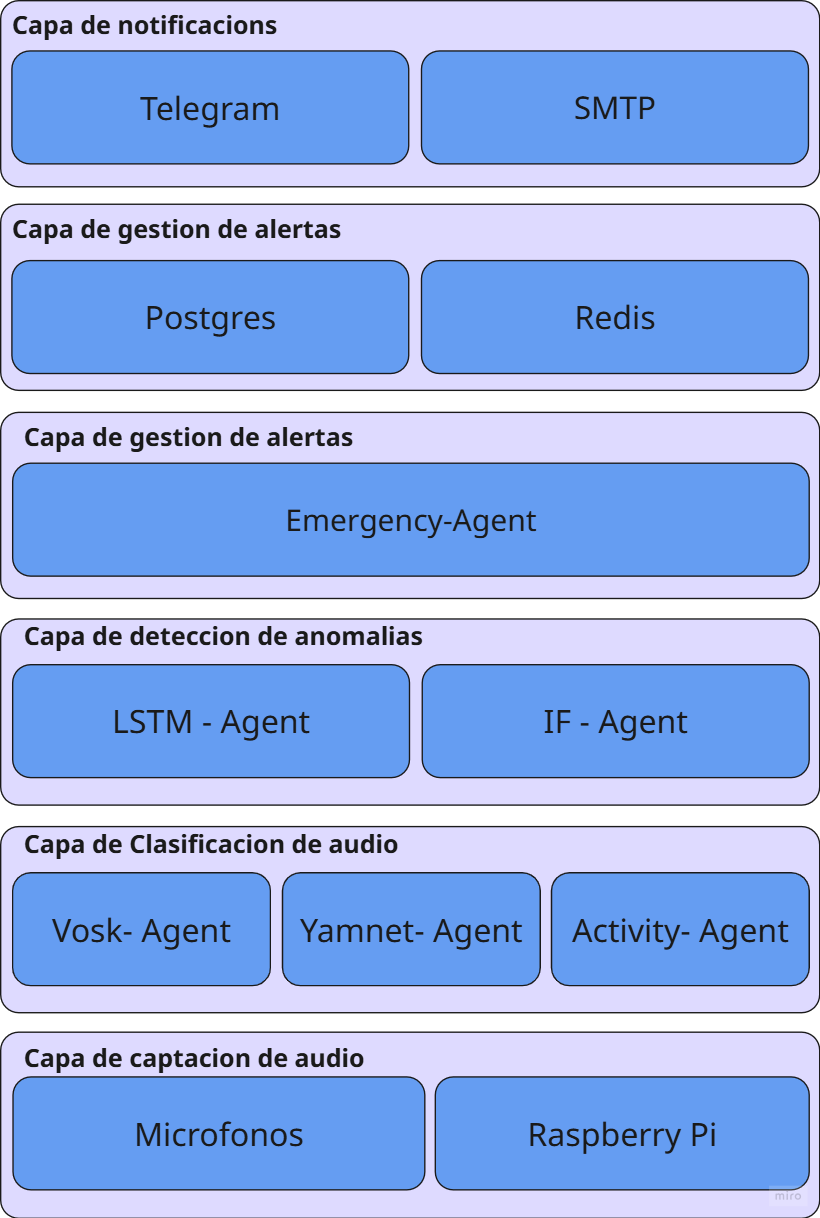
\includegraphics[width=0.40\textwidth]{Arquitectura/Arquitectura.png}
      \caption{Arquitectura del sistema de monitoreo acústico para generar alertas en casos de emergencia}
      \label{fig:arquitectura}
\end{figure}

\begin{enumerate}
      \item Capa de captación de audio: Esta capa corresponde al nivel más cercano al hardware y tiene como función principal la adquisición de datos acústicos mediante los micrófonos conectados al dispositivo Raspberry Pi. Se encarga de gestionar la interacción con el sistema operativo para acceder a las señales de audio en tiempo real y ponerlas a disposición del sistema a través de canales de comunicación internos. Su objetivo es abstraer la complejidad del hardware y garantizar que los datos se entreguen de forma continua a las capas superiores.
      \item Capa de clasificación de audio: Se encarga de analizar las señales acústicas recibidas de la capa de captación, tomando el flujo de audio en bruto como entrada para su procesamiento inmediato. En este nivel, múltiples agentes especializados (como Yamnet-Agent) procesan el flujo de audio con el fin de determinar la presencia de actividad, reconocer palabras clave y clasificar eventos característicos (como golpes, vidrios rotos o gritos) directamente a través de modelos preentrenados. Los resultados de este procesamiento se estructuran en mensajes que representan descripciones semánticas de la señal (es decir, una representación del sonido en términos de significado o evento), reduciendo drásticamente el volumen de datos y facilitando la interpretación, que se entiende como la traducción de datos brutos a eventos categorizados y listos para el análisis en etapas posteriores.
      \item Capa de detección de anomalías: En esta capa se aplican modelos de aprendizaje automático cuyos parámetros han sido fijados mediante un entrenamiento offline (como Isolation Forest y LSTM), pero que se ejecutan en tiempo real para la detección de anomalías. Utilizando los datos clasificados por la capa anterior como entrada, el sistema evalúa el comportamiento acústico observado de manera inmediata (online), diferenciando si este corresponde a patrones esperados o si representa una desviación significativa, como se demuestra con el cálculo del Mean Squared Error (MSE) en el LSTM-Agent. Esta capa constituye el núcleo analítico del sistema, ya que transforma datos objetivos en juicios de normalidad o anomalía en el momento en que ocurren. Si bien la detección de la anomalía es el objetivo principal de este nivel, el resultado debe ser complementado y validado por la Capa de Gestión de Alertas para añadir el componente contextual y la toma de decisión final.
      \item Capa de gestión de alertas: La función de esta capa es servir como el punto de decisión central del sistema, determinando cuáles de las anomalías detectadas deben ser escaladas como alertas finales al usuario. Si bien la implementación actual trata casi toda anomalía detectada por los agentes (Yamnet, LSTM, etc.) como una alerta inmediata, el diseño de la capa está basado en un mecanismo de validación y filtrado contextual. Este diseño aplica un conjunto de reglas (como la hora del día, el tipo de agente que emite la alerta o si el usuario ha pausado el sistema) y es crucial para el manejo de casos específicos, como la alerta por silencio prolongado en horario nocturno, o la interacción con el usuario mediante consultas verbales para validar la situación antes de enviar notificaciones externas. La existencia de esta capa asegura la preparación para la integración futura de variables contextuales adicionales (como detección de presencia o video) y garantiza la reduccion de falsos positivos a medida que se refinan las reglas de filtrado. Su propósito final es asegurar que solo las situaciones críticas, validadas contextual y/o humanamente, generen una respuesta definitiva.
      \item Capa de gestión de datos: Esta capa centraliza la persistencia y organización de la información recolectada y procesada por el sistema. Su propósito es almacenar los registros de eventos, tanto normales como anómalos, en estructuras que permitan su posterior análisis. Asimismo, prepara los conjuntos de datos necesarios para el reentrenamiento de los modelos de detección de anomalías, asegurando que el sistema pueda mejorar progresivamente su desempeño y adaptarse a nuevas condiciones acústicas en el entorno.
      \item Capa de notificaciones: Tiene como responsabilidad la comunicación con el usuario final o con sistemas externos de monitoreo. Actualmente, este módulo envía alertas validadas a través de servicios de mensajería como Telegram y protocolos de correo electrónico (SMTP). Su diseño es extensible, lo que permite incorporar otros canales de comunicación en el futuro. La existencia de esta capa garantiza que la información crítica llegue de forma oportuna a los responsables de la toma de decisiones.
\end{enumerate}

En la figura \ref{fig:arquitectura} se ilustra la arquitectura completa del sistema de monitoreo acústico, destacando las interacciones entre las diferentes capas y los agentes involucrados en el proceso de detección y notificación de anomalías.


\usubsubsection{Selección de hardware y dispositivos Edge}

Para la implementación del sistema, se realizó una evaluación de hardware con un enfoque en dispositivos de Edge Computing. La elección se centró en plataformas capaces de procesar datos localmente para reducir la latencia y la dependencia de la nube, como lo describen \citeauthor{shi_edge_2016} \citeyear{shi_edge_2016}. En este contexto, se seleccionó la Raspberry Pi como la plataforma de desarrollo, dada su versatilidad para integrar componentes como micrófonos y su amplia conectividad, características que la hacen ideal para aplicaciones de IoT y análisis en tiempo real según \citeauthor{richardson_getting_2016} \citeyear{richardson_getting_2016}.

La principal ventaja de este enfoque es que permite al sistema aprender las rutinas de su entorno específico, ya que los dispositivos permanecen fijos en un solo lugar. Esto requiere que los modelos de inteligencia artificial se ejecuten con los datos generados en dicho entorno. La alternativa (un gran servidor en la nube) sería muy costosa y poco práctica, pues exigiría mantener un modelo distinto para cada ubicación monitoreada, considerando que el sistema se compone de la interacción entre múltiples modelos. Por el contrario, un dispositivo edge como la Raspberry Pi resuelve este desafío al procesar los modelos localmente, permitiendo que cada unidad aprenda de manera autónoma sobre su entorno particular.

También se consideraron otros dispositivos edge, como el ESP32, pero se descartó debido a sus limitaciones de memoria y capacidad de procesamiento, que dificultarían la ejecución de modelos complejos de inteligencia artificial. Aunque el ESP32 es adecuado para tareas simples de detección de sonido basadas en umbrales, no cumple con los requisitos necesarios para implementar modelos avanzados como YAMNet o LSTM.

La comparación entre los distintos dispositivos edge se resume en el apendice C.


% \usubsection{Validación del sistema de monitoreo acústico para generar alertas en casos de emergencia}

% Para validar el funcionamiento del sistema de monitoreo acústico y su capacidad de generar alertas de emergencia, se procedió con un proceso de verificación. Este proceso se basó en el contraste directo del comportamiento del prototipo con los requerimientos operativos definidos, detallados en la Tabla \ref{tab:requerimientos_sistema_acustico}.

% La validación se concretó a través de la evaluación de los modelos de clasificación acústica en un entorno controlado mediante el uso de datos sintéticos. Se simularon escenarios acústicos, abarcando tanto condiciones de operación normal como eventos anómalos. El propósito fue verificar de manera objetiva si la salida del sistema, la clasificación del evento y la consecuente activación de la alerta correspondían con el resultado esperado, asegurando la correspondencia con su especificación.

% Los resultados obtenidos de esta verificación se consolidan en la Tabla \ref{tab:requerimientos_sistema_acustico}.